\chapter{Transition Rate Matrix Analysis} 
\label{sec:transRateChapter}
Now that we have MFT predictions about the relationship between density difference and
current in the SPM, it would be good to try to investigate their validity. In Chapter~\ref{sec:numerics} we will use Monte-Carlo methods to do this in $1$d and $2$d, but in this chapter we will restrict our attention to $1$d.

\section{The Transition Rate Operator for the SPM} \label{sec:TRMGeneralResults}
The SPM is an autonomous continuous-time Markov Process, which describes continual transitions between states
with transition rates depending only upon the current state. As such, if we call the total space of
states $\Xi$ then the probability distribution $P: \Xi \times \mathbb{R} \rightarrow  \mathbb{R}$ should obey a \textbf{master equation}
\begin{equation} \label{eq:masterEq}
 \partDeriv{P(\xi, t)}{t} = \mathcal{A} P(\xi, t),
\end{equation}
where $\mathcal{A}:\Xi \rightarrow \Xi$ is the \textbf{transition rate operator}
or TRO. Note that I am going to be using column vectors for probabilities rather than
row vectors, as many in the probability community do.
Parametrising $\mathcal{A}$ via 
\begin{equation}
 (\mathcal{A}f)(u) = \int_\Xi \! \! \mathrm{d}  \xi \ \sigma (u, \xi) f(\xi)
\end{equation}
puts it in a more familiar, transport equation-style notation:
\begin{equation}
 \partDeriv{P(\xi, t)}{t} = \int_\Xi \! \! \mathrm{d}  u \ \sigma (\xi, u) P(u, t) .
\end{equation}
Here $f: \Xi \rightarrow \mathbb{R}$ is an arbitrary function, intended to be a probability
distribution (nonnegative, unit measure, etc), whilst $\xi , u \in \Xi$ are dummy variables
and $\sigma: \Xi \times \Xi \rightarrow \mathbb{R}$ represents $\mathcal{A}$ in the basis 
determined by how we perform the integration.

We demand that $\sigma$ satisfies
\begin{equation}
 \forall \xi \in \Xi, \ \sigma (\xi , \xi) \le 0 
\end{equation}
and
\begin{equation}
 \forall \xi_1 , \xi_2 \in \Xi : \xi_1 \ne \xi_2 , \ \sigma (\xi_1 , \xi_2) \ge 0 ,
\end{equation}
as well as the constraint
\begin{equation}
 \forall u \in \Xi , \ \int_\Xi \! \! \mathrm{d}  \xi \ \sigma (\xi, u) = 0.
\end{equation}
The last constraint implies that
\begin{equation}
 \int_\Xi \! \! \mathrm{d}  \xi \partDeriv{P(\xi, t)}{t} = \int_\Xi \! \! \mathrm{d}  u \ P(u, t) \left[ \int_\Xi \! \! \mathrm{d}  \xi \ \sigma (\xi, u) \right] = 0
\end{equation}
regardless of the structure of $P$, which is our probability conservation equation.

The formal (forward-time) solution to Eq.~\ref{eq:masterEq} is given by
\begin{equation} \label{eqn:formalSoln}
 P(\xi, t) = e^{(t-t_0)\mathcal{A}}P_0,
\end{equation}
where $t_0$ is some initial time, $P_0$ is the starting distribution, and the operator
exponential is defined by its Taylor expansion, which should converge fine for bounded
$\mathcal{A}$, satisfied for the finite-system SPM. As 
$e^{(t-t_0)\mathcal{A}}$ and $\mathcal{A}$ share eigenvectors, we see that the
eigenstructure of $\mathcal{A}$ is something well worth investigating, as it should
give us information about the time-evolution of the system. An important thing to point
out is that $\mathcal{A}$ does not in general have orthogonal eigenvectors because it is
not in general symmetric,
and so we cannot normally diagonalise it using orthogonal transformations. This means that modes do not ``decouple'' in the way that states do in the 
Schr\"{o}dinger equation, and we instead have to deal with an \textbf{adjoint system}.

Luckily, when it comes to the analysis of steady states, there are a few results that
can help us. If we consider the operator $\mathcal{G}_T = e^{T\mathcal{A}}$ (in other words, the 
\textbf{propagator} for a period of time $T$), it is pretty easy to see that this is
a standard Markov Operator, as we are essentially reversing the limiting process
we would perform in order to define a continuous time Markov process as a limit of
a discrete time one. If we assume that $\Xi$ is finite and $\mathcal{G}_T$ is irreducible then as
a Markov operator it must possess  a unique eigenvector with corresponding eigenvalue $1$.
All other eigenvalues must have modulus between $0$ and $1$. Therefore, $\mathcal{A}$
must share that same unique eigenvector with associated eigenvalue $0$, and its other
eigenvectors must have negative real part. In physical terms, the system must have a single
steady state probability distribution, which it always relaxes towards exponentially
quickly, with a rate determined by the nonzero eigenvalue of $\mathcal{A}$ with real
part closest to $0$.

Of course, for such finite-state systems (such as the SPM on a finite domain) the integrals become sums, and $\sigma$ a matrix, $Q$. In such systems, we can arrange to have some labelling scheme which uniquely relates system states to natural numbers, and therefore
relates states to basis vectors in a vector space. In the SPM, a site is either full or empty, which means that there is a natural mapping between states and natural numbers based upon binary representation;
a string of $1$s and $0$s can be associated with a natural number as well as a configuration of particles and vacancies.

\subsection{A Small Worked Example: Closed System} \label{sec:workedExampleClosed}

As a concrete example, let us consider the SPM on a cyclic domain of length $3$. There
are $2^3$ possible combinations, and so $8$ possible states: $000$, $001$, and so forth.
The transition rate matrix describing this system is:
\begin{equation}
 Q =
 \begin{bmatrix}
0  &   &   &           &   &   &   &   \\
   &-2 & 1 &           & 1 &   &   &   \\
   & 1 &-2 &           & 1 &   &   &   \\
   &   &   & -2\lambda &   &  \lambda &  \lambda &   \\
   & 1 & 1 &           & -2&   &   &   \\
   &   &   &  \lambda    &   &  -2\lambda & \lambda  &   \\
   &   &   &  \lambda  &    & \lambda  & -2 \lambda &   \\
   &   &   &           &   &   &   & 0  \\
\end{bmatrix},
\end{equation}
where we have omitted most of the zero entries for clarity.
An alert observer will note that $Q$ is reducible, and so by permuting the basis vectors
we can rearrange the matrix into block form:
\begin{equation}
 Q ' = 
 \begin{bmatrix}
-2  & 1 & 1 &           &   &   &   &   \\
 1 &-2 & 1 &           &  &   &   &   \\
 1 & 1 &-2 &           &  &   &   &   \\
   &   &   & -2\lambda & \lambda &  \lambda &   &    \\
   &   &   &      \lambda& -2\lambda   &  \lambda &   \\
   &   &   &  \lambda   &   -2\lambda & \lambda & &   \\
   &   &   &       &  &  & 0 &  \\
   &   &   &           &   &   &   & 0  \\
\end{bmatrix}.
\end{equation}

According to our recipe, to learn about the solutions to Eq.~\ref{eq:masterEq} 
in this case, we need to know about the eigendecomposition of $Q$. 
The block structure of $Q'$ means that there are $4$ 
distinct parts of the state space, between which there are no transitions; this 
partitioning corresponds to the fact that particle number is conserved on the ring.
Two of these
sectors correspond to the full and empty states, and their dynamics are completely
trivial, in the sense that the state space is $1$d and there are no dynamics, as the
particles/vacancies have nowhere to go!
The remaining sectors correspond to the situation where there is one particle or one 
vacancy. The matrix is symmetric, meaning that its eigenvalues are real,
and we find that both nontrivial blocks can be diagonalised to form a multiple of
\begin{equation}
 \begin{bmatrix}
  0  &  &  \\
     &-3&  \\
     &  &-3\\
 \end{bmatrix},
\end{equation}
with eigenvectors $[1, 1, 1]^{\mathrm{T}}$, $[-1, 0, 1]^{\mathrm{T}}$ and
$[-1, 1, 0]^{\mathrm{T}}$ respectively, the latter two forming a degenerate eigenspace.

In this particular example then, we find that there $4$ steady states:
\begin{itemize}
 \item All slots full,
 \item All slots empty,
 \item One particle present, with equal chance to be in any particular position,
 \item The same but with a vacancy instead of a particle.
\end{itemize}
Whilst the first 2 cases are trivial (one-dimensional probability spaces), in the other
two cases we relax towards the steady state with rates $3$ and $3\lambda$ respectively.
In this example, the TRM was actually symmetric, and so all the eigenvalues were real.
It was also highly reducible, due to the strict constraints imposed by the particle
conservation law. When we have boundary conditions which permit the creation and
destruction of particles, that will change; we will consider that situation now.

\section{Forming the TRM for Systems with Dirichlet Boundary Conditions}

\subsection{Dirichlet Boundary Conditions} \label{sec:CTMPBoundaries}
In Chap.~\ref{sec:analChap} we made an MFT for the SPM in $1$-dimension, and when 
investigating steady states used Dirichlet boundary conditions when we needed them.
In particular, we had a system of length $L$ and sought solutions in which the system
density was pinned at $\rho_0$ at $x=0$ and $\rho_L$ at $x=L$. 

We would like to do a similar thing for the non-MFT SPM. An exact analogue of the situation
does not exist, as occupation number is not defined \textit{a priori} in a Markov process, but merely emerges as a result of the rate prescribed.The closest imitation to it
we can get is by allowing particles to be created and destroyed in boundary regions at
either end of a chain, and then try to set these rates so that the time-averaged occupation probability in the end sites are $\rho_0$ and $\rho_L$ respectively. Note
that this is a little more involved than simply loading and unloading particles as
one does in ASEP, as
\begin{itemize}
 \item loading and unloading really doesn't simulate the boundary condition we are looking for,
 which is attachment to a particle reservoir of constant particle density, and
 \item we actually need to consider a two-site boundary layer attached to each end, because the internal dynamics of the particles depend upon their immediate environment.
\end{itemize}
To simulate a boundary which is attached to a reservoir with occupation $\rho$, we allow
particles to appear in empty boundary sites with rate $B_0 \sqrt{\frac{\rho}{1-\rho}}$
and to disappear from full ones with rate $B_0 \sqrt{\frac{1-\rho}{\rho}}$,
for some positive $B_0$. If we switch
off all other dynamics and consider this in isolation, we would have a collection of
decoupled two-state systems. Writing a TRM for this with the first basis vector being
the empty state and the second the full one, we get
\begin{equation} \label{eq:blinkRates}
 Q = 
 \begin{bmatrix}
  - B_0 \sqrt{\frac{\rho}{1-\rho}} & B_0 \sqrt{\frac{1-\rho}{\rho}} \\
  B_0 \sqrt{\frac{\rho}{1-\rho}} & -B_0 \sqrt{\frac{1-\rho}{\rho}} \\
 \end{bmatrix}.
\end{equation}
There is of course a zero eigenvalue, which corresponds to a stationary distribution
$ [1-\rho, \rho]^\mathrm{T} $, precisely as desired.

In order to simulate attaching a reservoir with particle density $\rho$, we apply
the creation and annihilation rates above to the outermost two sites in our lattice.
The outermost site only performs these operations. The inner boundary site undergoes
these creation and annihilation processes, as well as the normal dynamics of the SPM;
thus, particles will move in and out of it as normal, and when the outermost site's
occupation is required to determine the transition rate for a particle moving inward,
that information is available. One could possibly eliminate the need for the outermost
boundary site by averaging over occupations, however we have chosen not to do this for
consistency with out Monte-Carlo calculations in Chap.~\ref{sec:numerics}.

Observant readers will notice that by using these creation and annihilation rates we
are left with a free variable, $B_0$. This controls the ratio of the creation and
annihilation rates to the internal dynamical rates $1$ and $\lambda$. In general
when we're trying to simulate an adjacent reservoir we want the boundary motion to be
``fast'' compared to the internal dynamics, and so $B_0$ may be regarded as a
regularisation parameter; any choice of $B_0$ should be good so long as
the creation and annihilation rates sufficiently dominate both $1$ and $\lambda$.
In practise, in our larger-scale calculations we  used
\begin{equation}
 B_0 = b(1+\lambda),
\end{equation}
with $b$ set to, $100$ or $1000$.

\subsection{Another Small Worked Example: Open System}

Using full boundary conditions, the smallest system we can consider consists of adjacent boundary
layers, in which particles pass directly from the inner layer of one boundary to the inner layer
of the other boundary. Unfortunately the state space of such a system is $2^4=16$-dimensional, and
so it would be cumbersome to consider such a system as an example here.

However, in the special case in which one boundary has density $\rho_0=1$ and the other has
$\rho_L=0$, the outer boundary layers become nondynamical, and the system simplifies considerably;
particles can only enter at the full end with rate $\lambda$, and can only leave at the empty end.
Therefore, we can consider a system consisting of single boundary layers attached to a single internal
slot without needing to consider a state space larger than $2^3=8$. Using the same state-labelling
convention as in Sec.~\ref{sec:workedExampleClosed}, the TRM for this new open system is
\begin{equation}
Q = 
\begin{bmatrix}
 -\lambda  & 1 &   &   &   &   &   &   \\
   & -\lambda -2 & 1 &   &   &   &   &   \\
   & 1 & -\lambda -2 & 1 & \lambda  &   &   &   \\
   &   &   & -2 \lambda -1 &   & \lambda  &   &   \\
 \lambda  &   & 1 &   & -\lambda  & 1 &   &   \\
   & \lambda  &   & \lambda  &   & -\lambda -2 & \lambda  &   \\
   &   & \lambda  &   &   & 1 & -\lambda  & \lambda  \\
   &   &   & \lambda  &   &   &   & -\lambda  \\
\end{bmatrix}.
\end{equation}
This time the matrix is not symmetric, and there does not exist a basis permutation which puts the
TRM into block form. If we calculate the characteristic polynomial $p(q) = |Q - q I|$, we find that
\begin{equation}
\begin{split}
 &p(q) = q \left[ q^7+(9 \lambda +7) q^6+\left(34 \lambda ^2+53 \lambda +17\right) q^5+\left(71 \lambda ^3+165 \lambda ^2+103 \lambda +17\right) q^4+ \right. \\
 &+\left(89 \lambda
   ^4+274 \lambda ^3+247 \lambda ^2+76 \lambda +6\right) q^3+\left(67 \lambda ^5+256 \lambda ^4+294 \lambda ^3+126 \lambda ^2+17 \lambda \right) q^2 \\
  &\left. +\left(28 \lambda ^6+127 \lambda ^5+171 \lambda ^4+91 \lambda ^3+15
   \lambda ^2\right) q + \left(5 \lambda ^7+26 \lambda ^6+37 \lambda ^5+24 \lambda ^4+4 \lambda ^3 \right) \right].
\end{split}
\end{equation}
Of course, the roots of $p(q)$ are the eigenvalues of $Q$. Clearly one of the eigenvalues is $q=0$,
and the others could be found by finding the root of the $7^\mathrm{th}$ order polynomial, which we
will not be doing analytically because it is extremely tedious and besides the point of this
example. The
$0$-eigenvector, and therefore the steady-state probability distribution over the possible
configurations, can be computed with a little care, and turns out to be
\begin{equation}
 q_0 = D^{-1}
 \begin{bmatrix}
  3 \lambda +1,\lambda  (3 \lambda +1) \\
  \lambda  (\lambda +2) (3 \lambda +1) \\
  \lambda ^3 (\lambda +3) \\
  (\lambda +3) (2 \lambda  (\lambda +2)+1) \\
  \lambda ^2 (\lambda +3) (2 \lambda +1) \\
  \lambda  (\lambda  (\lambda (\lambda +8)+14)+5) \\
  \lambda ^3 (\lambda +3) \\
 \end{bmatrix},
\end{equation}
where
\begin{equation}
 D = \lambda  (\lambda  (\lambda  (5 \lambda +26)+37)+24)+4.
\end{equation}
The variation of the occupation probabilities with $\lambda$ is displayed in
Fig.~\ref{fig:smallOccProbs}.
 \begin{figure}[h!]
 \caption[The variation of configuration probabilities with $\lambda$ for a small open system.]{\label{fig:smallOccProbs} 
 The variation of the steady-state configuration probability distribution with $\lambda$ for our
 open system. The coloured curves correspond to specific configurations, as indicated in the legend.
 }
  \begin{center}
 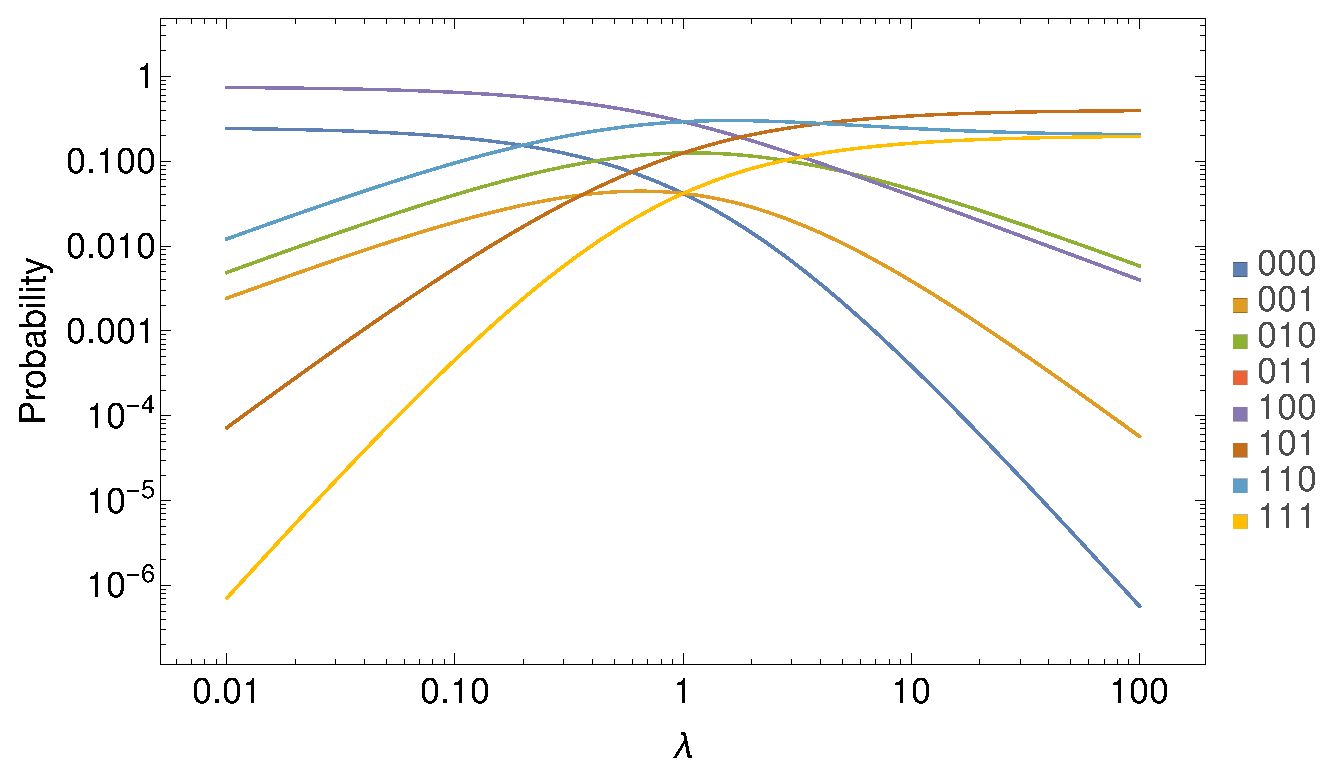
\includegraphics[width=1.0\textwidth]{TRM/images/smallOpenOcc}
  \end{center}
\end{figure}
Notice that at extremely small $\lambda$ the system either empties or a single particle gets stuck to
the full boundary, 
essentially preventing further flow by blocking it. Meanwhile, at large $\lambda$ there are
a few fairly popular states, with the most dominant being one with alternating particles and 
vacancies, as one might expect. The steady-state current from left to right in this system can be
calculated analytically once we have the steady state probability distribution, and turns out to be
\begin{equation}
 J = \lambda \left[ \frac{1}{4} + \frac{(1-\lambda)(3+\lambda)\lambda^2}{4+
 \lambda\left(24+\lambda\left[37+\lambda\left(26+5\right)\right]\right)}  \right].
\end{equation}
The second term in the bracket is generally dominated by the first, so we can say to an excellent
approximation that $J \sim \frac{1}{4} \lambda$. Thus, at least for this tiny example with very
extreme boundary conditions, there does not appear to be any change in the scaling of the current
with $\lambda$.

We can also compute the negative real part of the eigenspectrum of the TRM for this small system;
this is displayed in Fig.~\ref{fig:smallEigSpec}.
 \begin{figure}[h!]
 \caption[The variation of the eigenspectrum of the TRM with $\lambda$ for a small open system.]{\label{fig:smallEigSpec} 
 The variation of the negative real part of the eigenspectrum of the TRM for our small open system
 with $\lambda$.
 }
  \begin{center}
 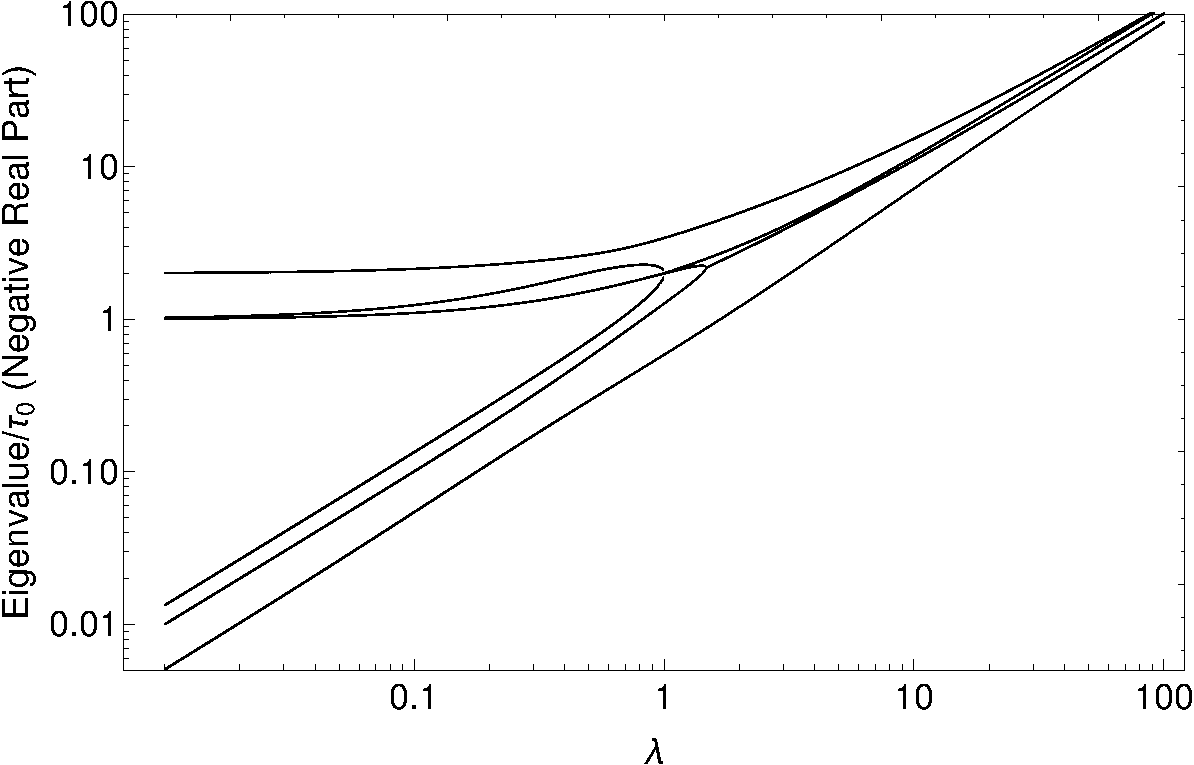
\includegraphics[width=1.0\textwidth]{TRM/images/smallOpenEigSpec}
  \end{center}
\end{figure}
It is in many ways rather similar to the eigenspectra we find for larger systems, so we see Sec.~\ref{sec:trmEigenspec} for our comments on those.

\subsection{Formation of the TRM in Sparse Format}

As we have seen, it is possible to find the eigendecomposition of the TRM analytically for extremely
small systems with special boundary conditions. However, we'd really like to see what happens for
somewhat larger systems, with more diverse boundary conditions. Thus, let us try to develop
a method for the numerical analysis of TRMs of arbitrary size.

The important thing to note about transition rate matrices for local lattice models
such as the SPM is that whilst the TRM itself grows very aggressively with system size, the TRM is generally extremely sparse.
The state space dimension grows as $2^L$, and the TRM dimension therefore grows as
$2^L \times 2^L$. However, a state containing $N$ particles only has transitions to
\begin{itemize}
 \item states which differ from the current state by one particle move, of which there
 are $\mathcal{O}(N)$, and
 \item states which differ from the current state by a single particle creation or
 annihilation, of which there are $\mathcal{O}(4)$.
\end{itemize}
Thus, as $N \le L$ the number of nonzero entries in the matrix is 
$\mathcal{O}(2^{L}L)$,
which is not a particularly tight bound. Therefore, the overall density of the TRM
is $\mathcal{O}(2^{-L}L)$. Given that there already exist a great many efficient
numerical routines for sparse linear algebra operations, there exists the possibility
that we could use this to solve the SPM on a finite domain for small systems
``exactly'' (or at least, up to some nominated numerical tolerance).

To make use of this, we need to assemble the TRM in a suitable sparse format.
I have written a Python code which does this. The script itself is stored <decide how 
precisely>, but the gist of the algorithm is to simply run through all possible states,
document all the transitions they can perform, and store the resulting entries in
a sparse matrix element by element. During construction, the matrix should be stored in
coordinate list format, i.e. a list of elements of the form $(\mathrm{row}, 
\mathrm{column}, \mathrm{value})$, as this is trivial to update as we only inspect
each matrix entry once. We can then convert the matrix to a compressed format such
as CSC (Compressed Sparse Column) or CSR (Compressed Sparse Row). We used CSC, but in
hindsight CSR would probably have been a better choice as it tends to make
matrix-vector multiplication a little more efficient. Once we have the TRM in this
format, it is ready for sparse linear algebra operations. Note that whilst
these operations generally happen ``in place'', this part of the process is the
memory-intensive bit, as of course the memory usage scales with the number of nonzero
matrix elements, which is $\mathcal{O}(2^{L}L)$.
In terms of actual numbers, we found
that 4Gb of memory was more than adequate to solve a system of $16$ sites in total.
As the memory required to represent the TRM is the main limiting factor in this kind of
calculation, if we were to attempt a larger calculation we would probably switch to using a
machine with a very large working memory, such as DiRAC.

\section{The Eigenspectrum of the TRM}

\subsection{The Computation of the TRM Eigenspectrum} \label{sec:eigenFind}
Once we have the TRM $Q$ in CSC or CSR format, we can then use sparse linear algebra. 
In our code we called the Python routine \texttt{scipy.sparse.linalg.eigs} upon it,
which itself is a wrapper for C codes which find eigenpairs according to desired
criteria; precisely which algorithm to used is determined during runtime, and it may
try different methods if it doesn't initially succeed.

In our computations, we typically performed two types of calculation. In the first we merely sought to
find the steady state, so which we requested only the eigenvector $x_0$
associated to the
eigenvalue $q_0$ with smallest absolute value, which should always be numerically zero.
We requested that the eigenpair be found to a relative accuracy $\epsilon$ accuracy of $1$ part in $10^{12}$,
which amounts to saying that
\begin{equation} \label{eq:linAlgRelAcc}
 \frac{\| Q x_0 - q_0 x_0 \|}{\| x_0 \|} \le 10^{-12} = \epsilon
\end{equation}
where $\| \cdot \|$ is some reasonable subordinate matrix norm (in our case, the $1$ norm). Because we requested the eigenvalue closest to $0$, \texttt{eigs} used the
shift-invert method <find article>, leading to greater accuracy in the computation of
eigenvalues near to $0$ which is exactly what we wanted. For the other type of
computation, we instead requested the $k$ eigenpairs with largest real part, which
most likely provoked the code to use a Implicitly Restarted Arnoldi Method (IRAM).
This is not as accurate for computing the steady state, but yields vastly more accurate
results when computing the other eigenpairs compared to the first method. 

\subsection{The Structure of the TRM Eigenspectrum} \label{sec:trmEigenspec}

Using the code listed at <place>, we can compute the eigenspectrum of an SPM system
with boundary densities connected at both ends. Such a computation requires the
following parameters to be specified:
\begin{itemize}
 \item $\rho_0 \in (0, 1)$, the density of the reservoir connected to the left end of the domain.
 \item $\rho_L \in (0, 1)$, the density of the reservoir connected to the right end of the domain.
 \item $L \in \mathbb{N}$, the system size.  The way we have defined things in the code, we do not
 count the two sets of two particles representing the boundary; thus, $L=1$ actually
 refers to a system which contains $5$ lattice sites, of which $4$ are busy doing
 boundary duties.
 \item $b>0$, the variable which controls the separation of timescales between the 
 flickering motion on the boundaries and the internal motion within the bulk of the
 system. This should be set to something large, and compared to other values of it
 to ensure that it is working as a regularisation parameter
 (i.e. large changes to $b$ have minimal impact on the relevant internal
 dynamics of the system, even if they have a great impact on the boundary dynamics).
 \item $\lambda>0$, the internal anomalous movement rate in the SPM.
 \item $\epsilon$, the relative accuracy the calculation aims for in the sense of Eq.~\ref{eq:linAlgRelAcc}.
 \item $1 \le k < 2^{L+4}$, the number of eigenvalues to compute.
 \end{itemize}

 For consistency we kept $L$, $b$, $\epsilon$ and $k$ constant during runs of 
 calculations. This leaves $\rho_0$, $\rho_L$ and $\lambda$ to be varied. In terms of what to vary and how to display the data, we decided to
 allow the spectrum to depend upon only one variable, and picked $\lambda$ to be that
 variable. We generally chose $\rho_0 =0.6$ and $\rho_L =0.4$ in order to study a system in which,
 at least for $\lambda=1$, the density is middling and a current flows.
 We then computed the resulting eigenspectrum in a couple different ways.
 First, we performed a relatively small calculation, in terms of the number of eigenvalues demanded and the number of $\lambda$ used. We altered the values of $L$
 and $b$ between runs, so that we can see what impact they have on the eigenspectrum. We then performed a very
 large calculation, in order to get a good look at the eigenstructure as a whole.
 In Chap.~\ref{sec:analChap} our MFT suggested that a transition might occur around
 $\lambda=\frac{1}{4}$, so we should look out for odd behaviour in that regime.

 To actually perform these TRM calculations, we used Edinburgh Compute and Data Facility's Linux
 Compute Cluster, known as Eddie3. We will discuss this machine and its capabilities further in
 Chapter~\ref{sec:numerics}. Although we did initially consider the possibility of exploiting the natural parallelisability of the numerical linear algebra routines, we concluded that it
 was not probably not worthwhile in terms of computational gains, whilst requiring a lot of
 extra development time to implement. Instead, we simply submitted large numbers of separate serial
 jobs with different parameter values (e.g. for $\lambda$, $\rho_0$, $\rho_L$) to Eddie3, and then
 allowed the machine to process them in its own time.
 
 \subsubsection{Small Calculations}
 First, we performed a calculation with $L=5$, $b=1000$ in which we computed the
 negative real part of the $32$ eigenvalues with real part closest to zero for a wide range of $\lambda$ with fixed
 boundary conditions. The resulting eigenspectrum is displayed in
 Fig.~\ref{fig:eigsL5B1000}.
 \afterpage{
 \begin{figure}[!ht]
 \caption[The TRM eigenspectrum for a system with $L=5$, $b=1000$.]{\label{fig:eigsL5B1000} 
 The TRM eigenspectrum, computed for a system with $\rho_0 = 0.6$, $\rho_L = 0.4$,
 $L=5$, $b=1000$.
 }
  \begin{center}
 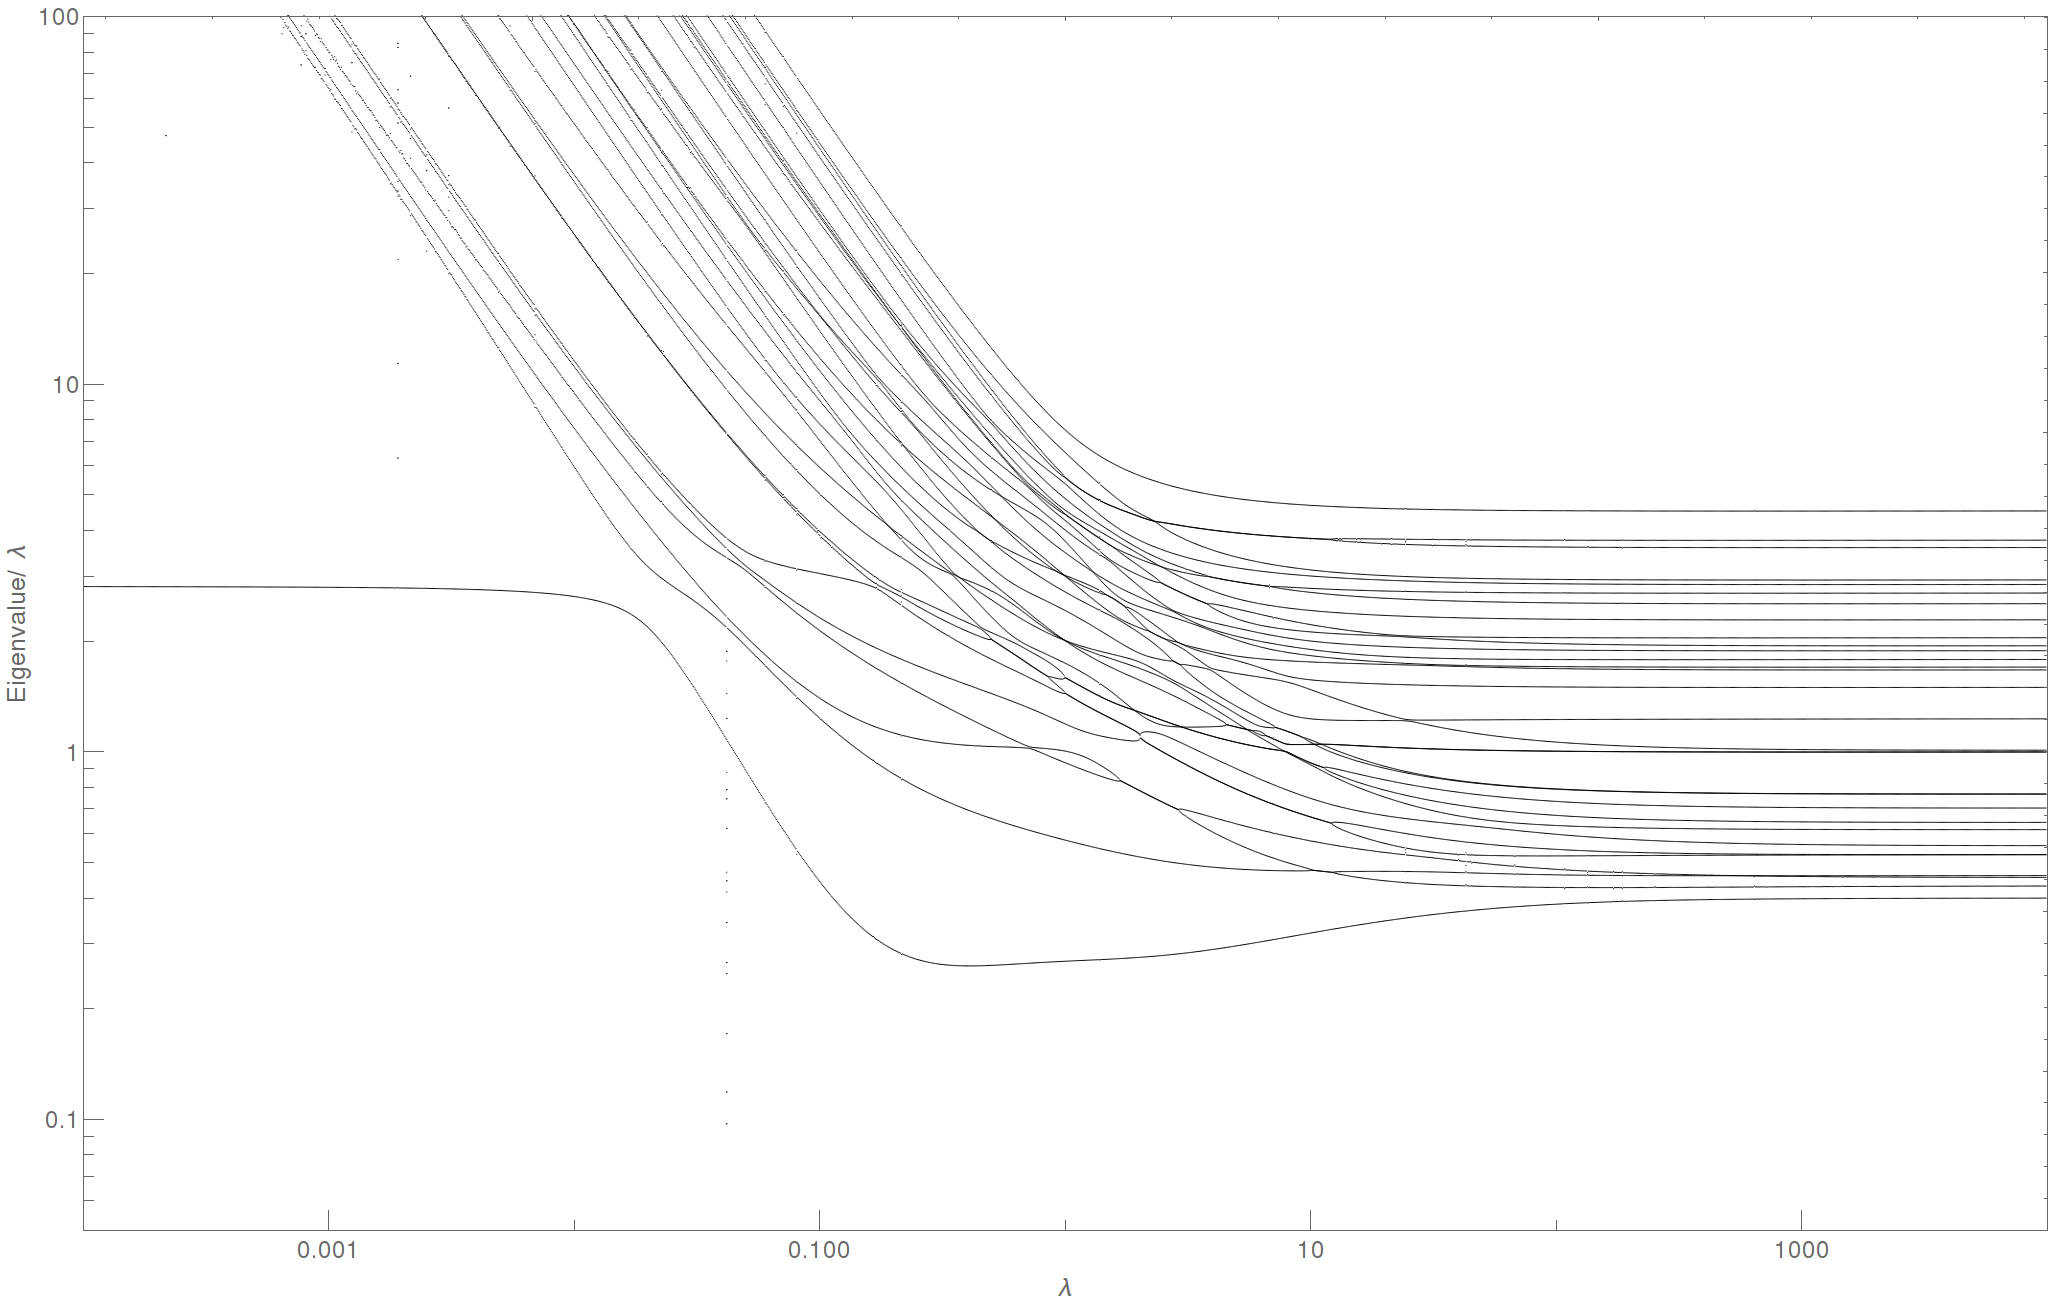
\includegraphics[width=0.9\textheight, angle=270]{TRM/images/singleMultEigB1000L5}
  \end{center}
\end{figure}
\clearpage
}
Of course, for such a system we expect that all eigenvalues have negative real part,
as we discussed in~\ref{sec:TRMGeneralResults}, so we have chosen to plot the
negative real part divided by $\lambda$ as a function of $\lambda$; the zero eigenvalue,
which we expect to exist and is generally found to exist in numerical terms, has been ignored, as its magnitude is simply an artefact of the numerical calculation and
is therefore meaningless except possibly as a check on the numerics. The decision 
to divide by $\lambda$ was taken because the eigenvalue closest to $0$ (which dominates
approach to equilibrium) mostly scales as $\mathcal{O}(\lambda)$, so plotting without division
uses graph space poorly.

There are a several things to note about this spectrum:
\begin{itemize}
 \item It would appear that, for all $\lambda$, there is a single eigenvalue which
 is closest to $0$ and undergoes no definitive crossing as $\lambda$ varies. At both extremes of
 $\lambda$, it clearly scales as $\mathcal{O}(\lambda)$, but is unusually low in an intermediate regime of $\lambda \in (0.03, 10)$, reaching a minimum at $\lambda \sim 0.3$, which could be
 interpreted as an ``avoided crossing'' with the 0-eigenvalue. This is
 important, as the eigenvalue with smallest negative real part is the one that controls
 the approach to equilibrium; thus, we can see that around $0.3$ the system should taken unusually long to relax from an arbitrary prepared state to equilibrium.
 \item All eigenvalues tend to scale as $\mathcal{O}(\lambda)$ as $\lambda \rightarrow \infty$.
 \item Eigenvalues other than the bottom one tend to scale as $\mathcal{O}(1)$ at small
 $\lambda$. Thus, whilst the overall approach to equilibrium occurs with rate 
 $\mathcal{O}(\lambda)$, there are still plenty of (probably more localised) processes 
 occurring over much quicker timescales, whilst the whole system is sluggish to 
 equilibrate.
 \item The eigenvalues tend to retain their order at the extremes of $\lambda$, 
 but they frequently cross, merge and separate again in the intermediate regime. This suggests that something complicated is occurring; an analytic solution to this dynamical model would need to describe these crossings in detail, as they are important as
 eigenvalue crossing implies the appearance of degenerate eigenspaces in the decay modes
 which the associated eigenvectors refer to. This makes it look rather 
 unfeasible that such an analytic solution could be constructed in the first place.
\end{itemize}
Of course, this is only the $32$ lowest eigenvalues; there could be different behaviour
in the higher ones. Before we perform a larger calculation however, let us turn our
attention to the dependence of the eigenspectrum upon $b$ and $L$, which we have studied
by repeating our calculation with different values for those parameters, as shown in
Fig~\ref{fig:eigsVarBVarL}.
\afterpage{
 \begin{figure}[h!]
 \caption[The lower part of the TRM eigenspectrum for a system with $L=\{5, 10\}, $, $b=\{100, 1000\}$.]{\label{fig:eigsVarBVarL} 
 The lower TRM eigenspectrum, computed for a system with $\rho_0 = 0.6$, $\rho_L = 0.4$,
 with all combinations of
 $L=\{5, 10\}$, $b=\{100, 1000\}$. Missing computations, visible via the vertical gaps in
 the data, are due to computational issues, rather than being numerically meaningful. Note that
 in many places green/black and blue/red lines overlap, because their results are so similar; the
 image is deliberately prepared in a high resolution so that these intricacies may be observed,
 at least in the digital copy.
 }
  \begin{center}
 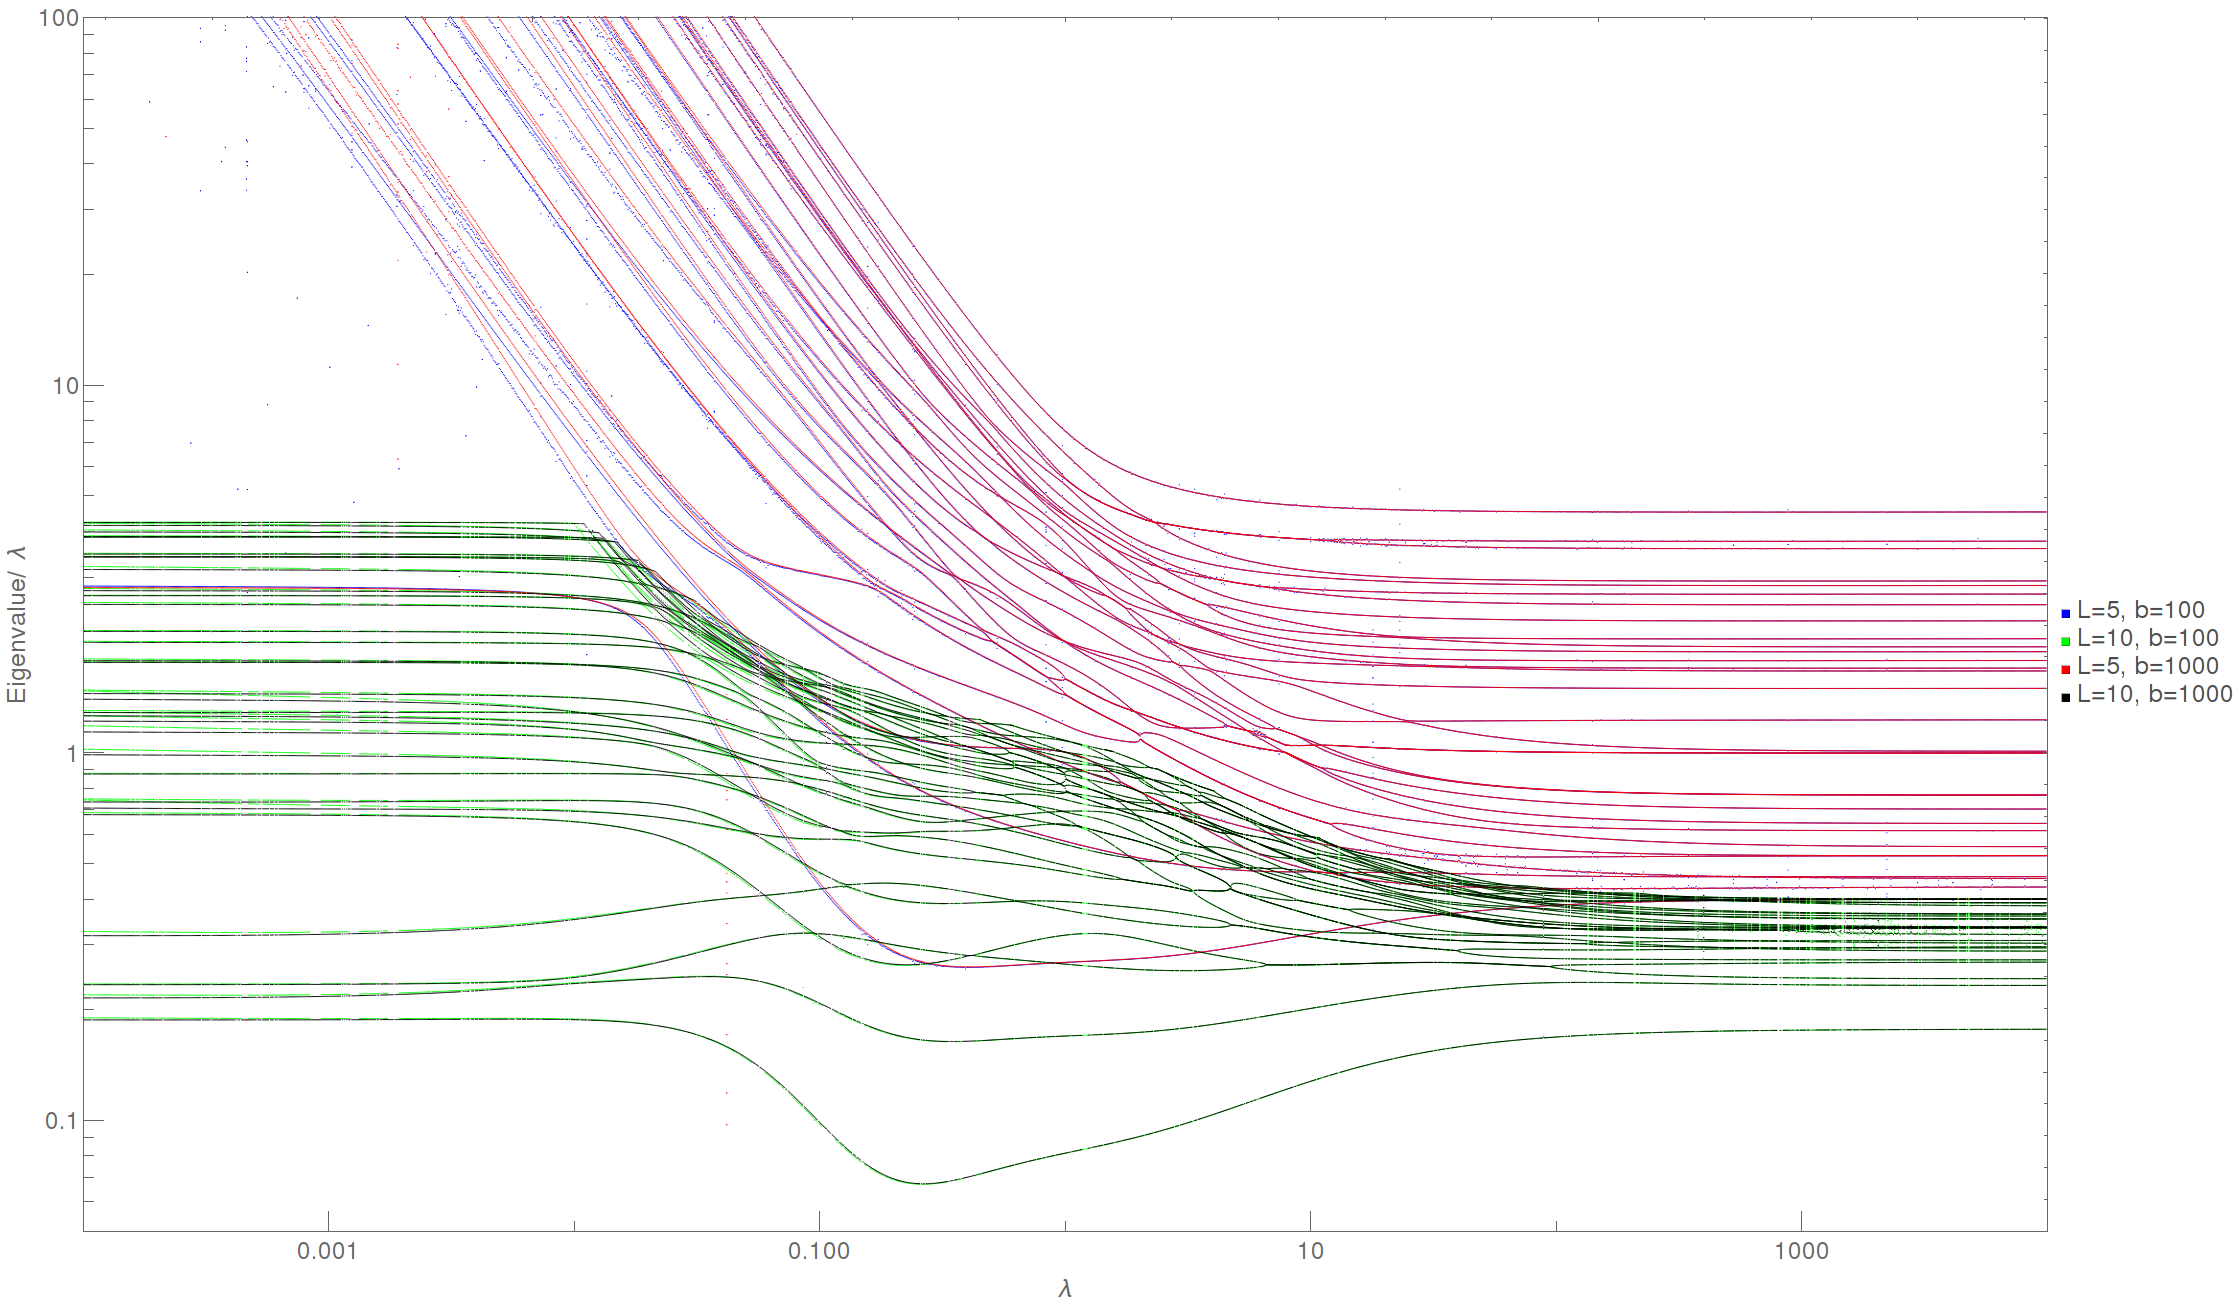
\includegraphics[width=1.0\textheight, angle=270]{TRM/images/repeatRepeatMultEig}
  \end{center}
\end{figure}
\clearpage
}
Again, there's a lot going on in this image, so let's break it down.
\begin{itemize}
 \item Firstly, let us note that keeping $L$ constant and switching $b$ between $100$
 and $1000$ seems to have very little impact on the eigenspectrum, as we can see by the fact that the points corresponding to the same system sizes are
 more or less lying on top of each other unless we delve into the low-$\lambda$ limit
 of the $L=5$ system. In the same limit, we see that the discrepancy is vastly reduced
 in the $L=10$ system, suggesting that it is less bad for large systems, and is in some sense a small-size effect. Regardless, it would appear to be the case that adjusting $b$
 doesn't affect these low-lying eigenvalues very much, so it seems to be playing its
 role as a regularisation parameter as intended. Thus, we're simply going to use $b=1000$
 from now on, unless explicitly specified otherwise.
 \item The bottom eigenvalue, which controls relaxation to equilibrium, is generally
 several orders of magnitude lower for the $L=10$ system than for the $L=5$ one;
 this effect is particularly extreme in the limit of small $\lambda$.
 This makes sense; the larger system should take much longer to equilibrate than the
 smaller one, as so many more fluctuations need to occur to make it change its global
 state. This is something we should remember for later, as it suggests that equilibration time might scale
 pretty aggressively with system size, which is bad news for our attempts to simulate
 the system using Monte-Carlo methods (Chap.~\ref{sec:numerics}).
 \item The big, obvious difference between the spectra of different system size is
 the behaviour at small $\lambda$. For $L=5$ there is only $1$ eigenvalue which scales
 as $\mathcal{O}(\lambda)$ as $\lambda \rightarrow 0$, whereas for $L=10$, it would
 appear that they all do!
\end{itemize}
The last point begs the following question: how does the number of eigenvalues
corresponding to ``slow modes'' at small-$\lambda$ scale with the system size? This is 
important,
because it determines how many of the available decay modes would tend to persist for any 
meaningful amount of time during the relaxation towards equilibrium. We will attempt to
address this in the next subsection.

\subsubsection{The Scaling of the Number of Slow Modes at Low $\lambda$}
To find out how the number of nonzero eigenvalues in the $\mathcal{O}(\lambda)$-scaling
band (as observed in Fig.~\ref{fig:eigsVarBVarL}) scales with system size,
we can simply fix $\lambda$ to be sufficiently low (say, $\lambda=0.0001$)and repeat
computations of the low-lying eigenspectrum for different $L$. Here, due to the
computational limitations we are up against, we only compute up to $L=13$. The number
of slow modes as a function of $L$ is displayed in Tab.~\ref{tab:bandThickness}.
\begin{table} \caption[Tabulated values for the variation of the width of the slow band with
system size.]{A table of the number of slow modes occurring at low $\lambda$ for given 
$L$.}
\begin{center}
\begin{tabular}{r || r | r | r | r | r | r | r | r | r | r | r | r} \label{tab:bandThickness}
 $L$ & 5 & 6 & 7 & 8 & 9 & 10 & 11 & 12 & 13 \\
 \hline
 Bandwidth & 1 & 3 & 6 & 11 & 20 & 36 & 64 & 113 & 199 \\
\end{tabular}
\end{center}
\end{table}
If we plot the number of slow modes as a function of system size on a plot with a 
logarithmic $y$-axis, as we have done in Fig.~\ref{fig:bandWidthScaling},
it is rather obvious that the bandwidth scales exponentially with system size.
However, the number of slow modes seems to scale as $\mathcal{O}(2^{\sim 0.84 L})$,
whereas the number of possible states, and therefore the total number of eigenvalues of
the TRM, scales as $2^L$. Thus, one can see that although the number of slow modes grows
very aggressively with the system size, it would appear to eventually become 
outpaced by the growth in the total number of eigenvalues; in this way, we can say that
the slow band carries increasingly less of the total eigenvalue density as system size
becomes large.
 \begin{figure}[h!]
 \caption[A graph of the scaling of the number of slow modes with system size.]{\label{fig:bandWidthScaling} 
 A plot of the scaling of the number of slow modes in the eigenspectrum of the TRM of
 an SPM system of size $L$. The trendline displayed has equation
 $ \mathrm{Bandwidth} = 2^{a(L+b)}$, with $a=0.84$, $b=-3.9$.
 }
  \begin{center}
 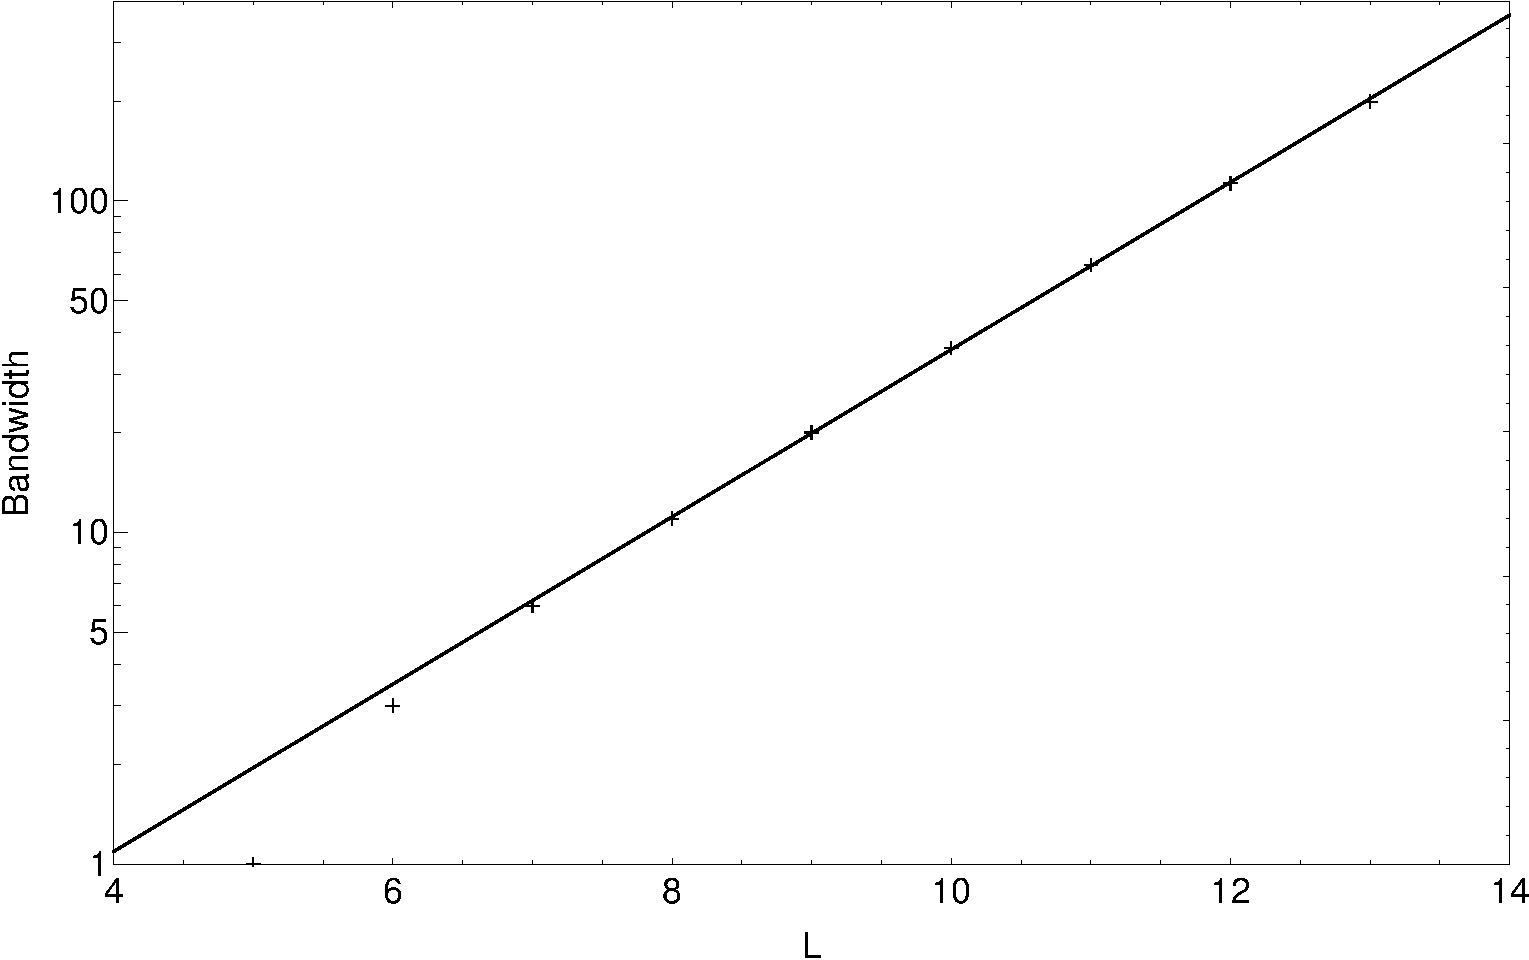
\includegraphics[width=1.0\textwidth]{TRM/images/bandWidth}
  \end{center}
\end{figure}

\subsubsection{The Upper Part of the Spectrum}

By varying $L$ and $b$ and analysing the lower (more physically relevant) part of the
TRM eigenspectrum, we concluded that $b$ has very little impact and essentially
acts as a regularisation parameter, whilst $L$, the system size, has a large impact,
particularly on the approach to equilibrium. However, both $b$ and $L$ contribute to
the actual numbers contained within the TRM, so it stands to reason that they must
impact the eigenspectrum in some way. Therefore, we have done an additional check,
by varying $b$ and $L$ and 
performing a calculation in which the $64$ eigenvalues with largest negative real
part were calculated. The negative real parts of these eigenvalues are displayed in
Fig.~\ref{fig:eigsVarBVarLUpper}.
 \begin{figure}[h!]
 \caption[The upper TRM eigenspectrum for a system with $L=\{5, 10\}, $, $b=\{100, 1000\}$.]{\label{fig:eigsVarBVarLUpper} 
 The upper TRM eigenspectrum, computed for a system with $\rho_0 = 0.6$, $\rho_L = 0.4$,
 with all combinations of
 $L=\{5, 10\}$, $b=\{100, 1000\}$.
 }
  \begin{center}
 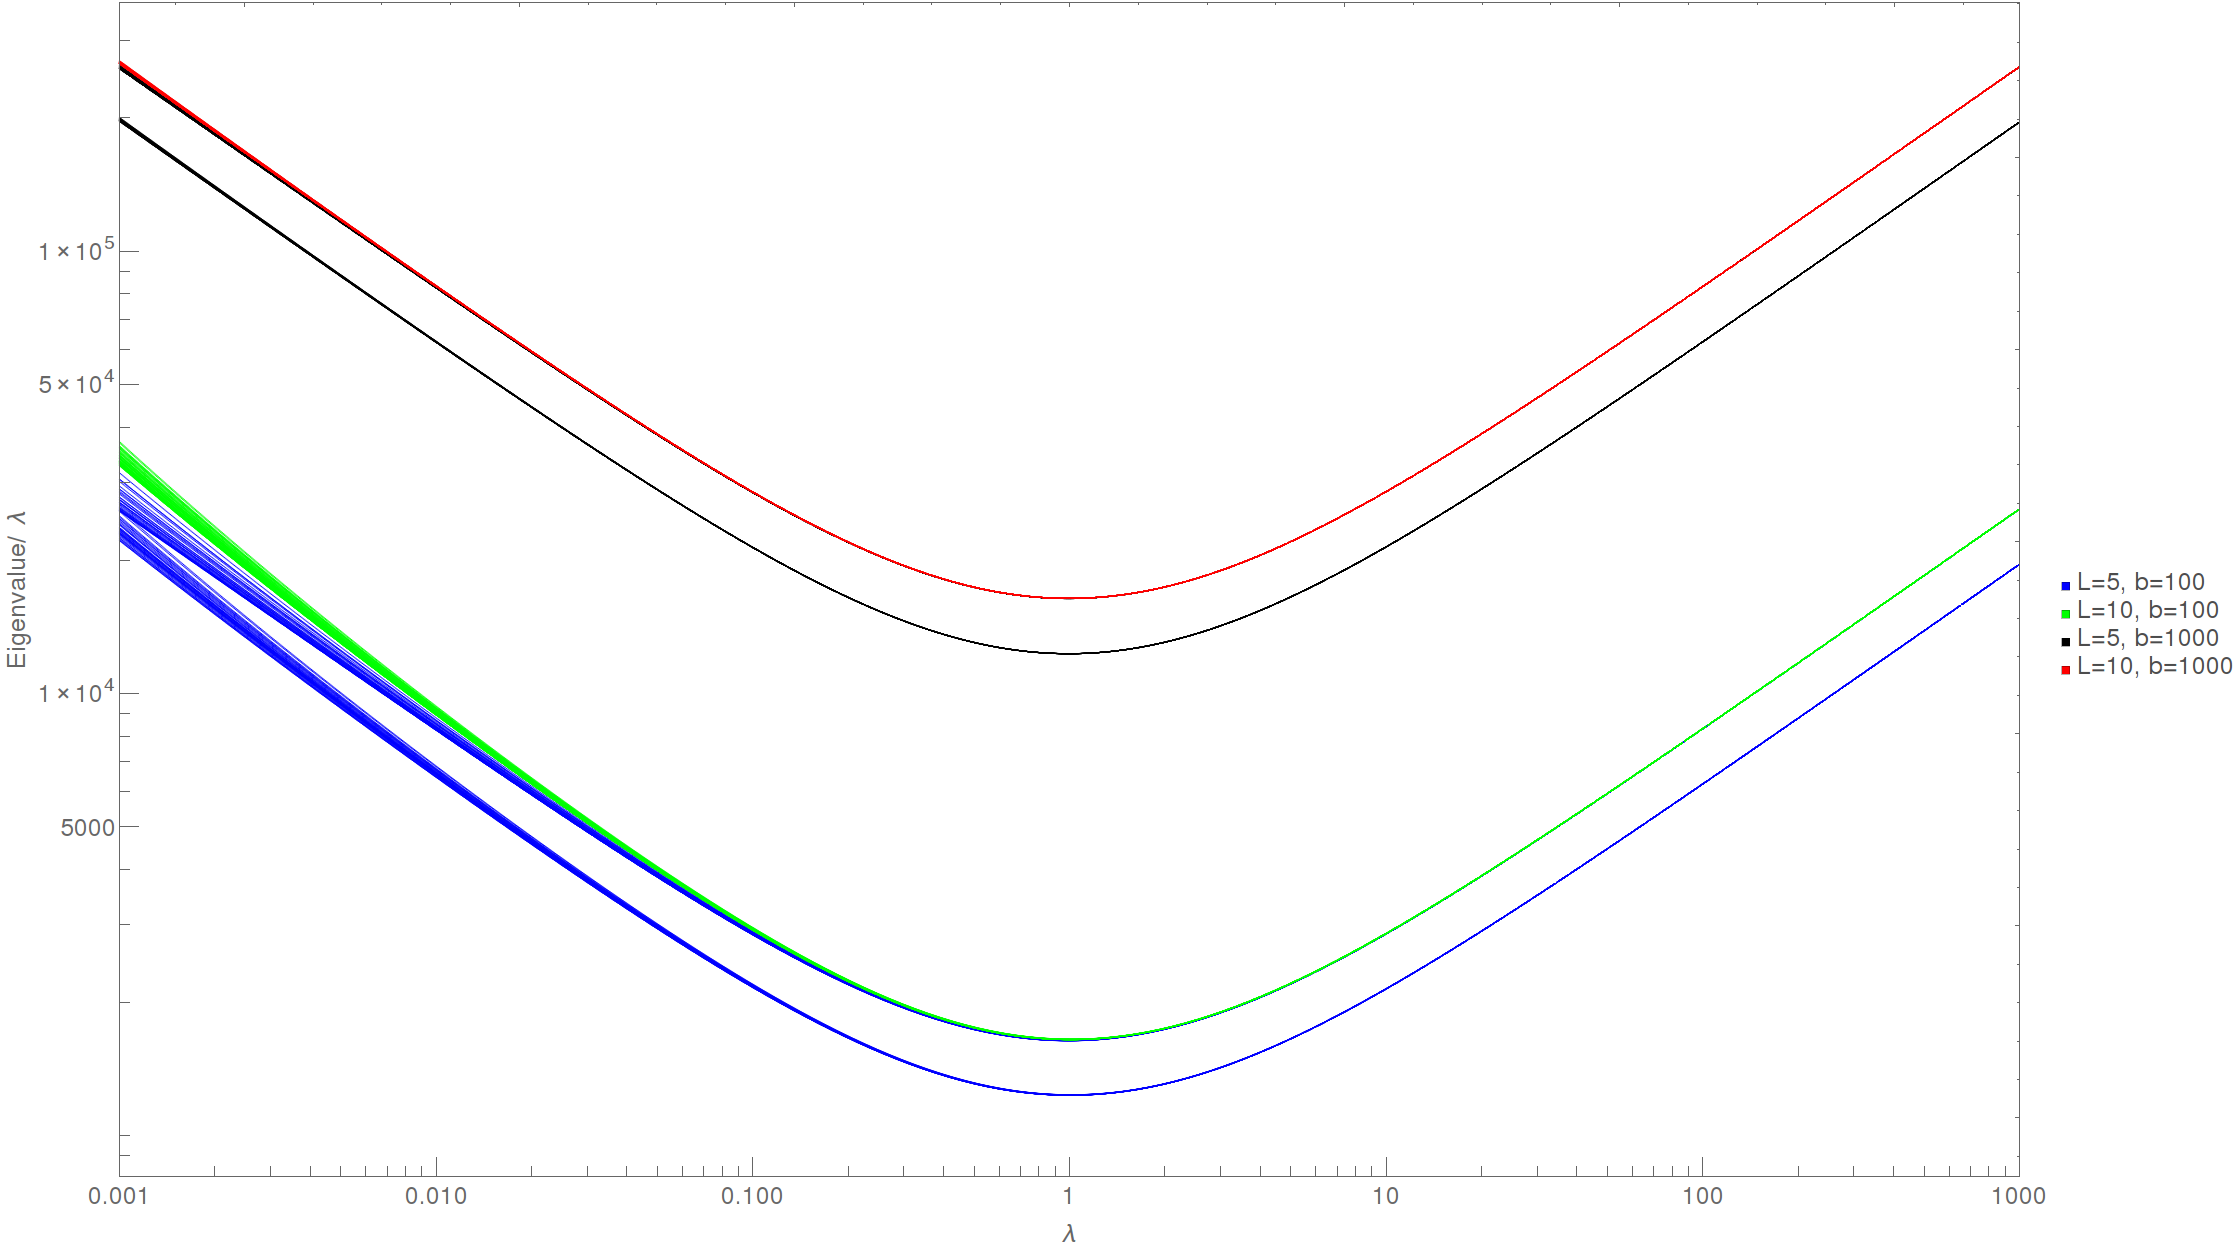
\includegraphics[width=1.0\textheight, angle=270]{TRM/images/topEigs}
  \end{center}
\end{figure}
We see that now the tables are indeed turned. Altering $L$ does have a small effect on
the upper band, as we can see by how the red/black and blue/green points lie on top
of each other. On this graph, we see that for the $L=5$ datasets there are apparently
two bands, whilst for $L=10$ there is only one; however, recall that we have produced
this by plotting the negative real parts of the $64$ eigenvalues with largest negative
real part; thus, as the $L=10$ systems have $2^5 = 32$ times as many eigenvalues in 
total, it makes sense that we may not have finished the very top band in the $L=10$
case yet whilst we have moved on to the second band in the $L=5$ case; thus, we conclude that
system size has little effect on the top of the eigenspectrum.

The value of $b$, however, has a huge impact, as it determines the overall magnitude
of these larger eigenvalues. The eigenmodes associated with them almost certainly
relate to fluctuations at the boundary, and then the ensuing joint fluctuations 
travelling a little into the bulk. As these are boundary effects, it again makes sense
that $L$ has little impact. The value of $b$ directly controls the speed of the 
fluctuations at the boundary, thus the large shift in magnitude observed should be 
expected.

\subsubsection{Large Calculation}
Now that we are more or less satisfied that the value of $b$ doesn't matter so long as
it's quite large, let's perform a similar calculation (sweeping through $\lambda$ with
constant boundary conditions), but this time compute a lot of eigenvalues in order to
get a general overview of the TRM. 
\afterpage{
 \begin{figure}[h!]
 \caption[The ``full'' TRM eigenspectrum for a system with $L=8, $, $b=1000$.]{\label{fig:bigEigSpec} 
 The ``full'' TRM eigenspectrum, computed for a system with $\rho_0 = 0.6$, $\rho_L = 0.4$,
 with $L=8$, $b=1000$. Missing computations, visible via the vertical gaps in
 the data, are due to computational issues, rather than being numerically meaningful.
 }
  \begin{center}
 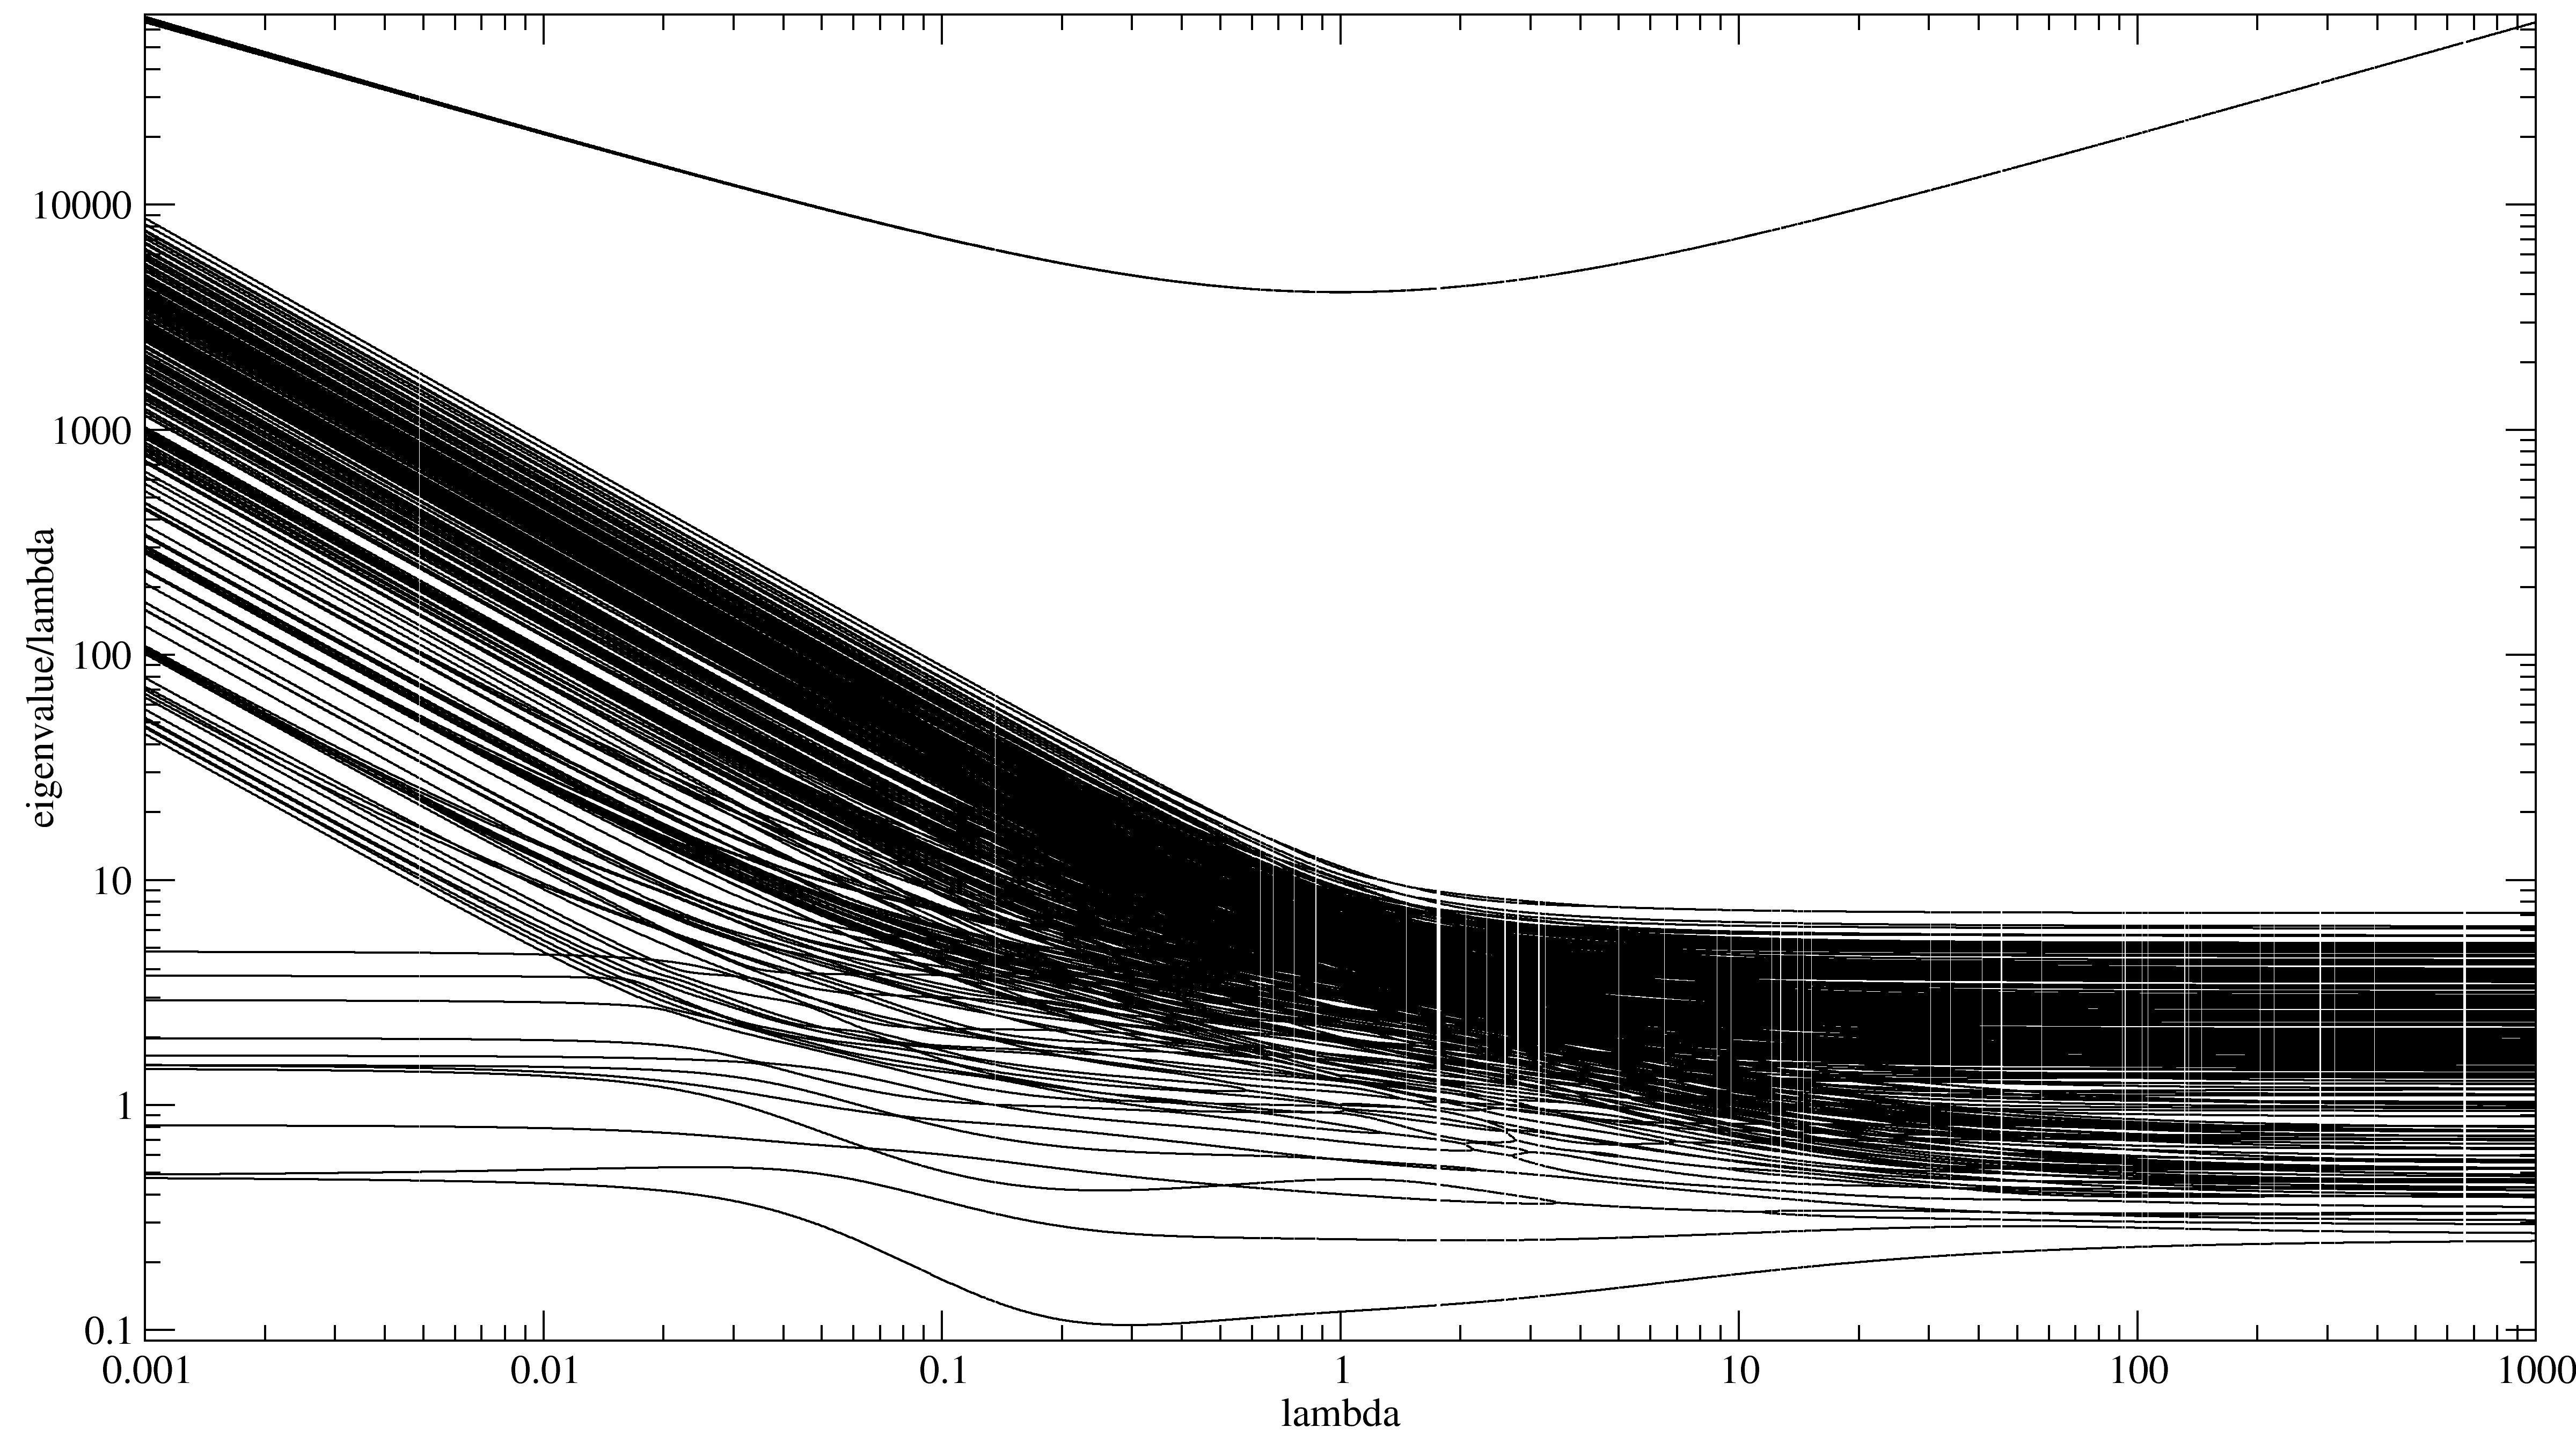
\includegraphics[width=0.9\textheight, angle=270]{TRM/images/bigEigSpec}
  \end{center}
\end{figure}
\clearpage
}
Plotted in Fig.~\ref{fig:bigEigSpec} are the negative real components of the $1024$ eigenvalues with smallest negative
 real part, for the TRM of an SPM system of length $L=8$ and regularisation parameter 
 $b=1000$. We say that this is the ``full'' eigenspectrum not because
 we have computed all of the eigenvalues (we have not, as there are $2^{12} = 4096$ in
 total), but because the eigenvalues with very large negative real part seem to converge
 upon each other, forming the hyperbola-shaped entity towards the top of the graph.
 We believe that this is because the relevant dynamical modes correspond to extremely rapid changes in system state which are limited to the region immediately around the boundaries; as these should
 have no impact on large-scale properties such as the current, they are of very limited
 interest
 to us.
 
This large computation continues the themes we have seen in the small ones:
\begin{itemize}
 \item For large $\lambda$ there is a thick band of eigenvalues spread over a couple
 of orders of magnitude which scale as $\mathcal{O}(\lambda)$.
 \item For intermediate $\lambda$ the bottom eigenvalue becomes unusually small, whilst
 the higher ones in the thick band are constantly crossing over each other.
 \item As we go to small $\lambda$ a thin band of $\mathcal{O}(\lambda)$-scaling
 eigenvalues split off from the main sequence, which scales as $\mathcal{O}(1)$.
 \item For all $\lambda$ there is the hyperbola-shaped band of eigenvalues with highly
 negative real part, which are many orders of magnitude different to the main sequence;
 thus, their dynamics operate over an extremely short timescale, and they are almost
 certainly attributable to the flickering motion at the boundaries.
\end{itemize}



\subsection{Current and Density in the Steady State}
The eigenvectors of the TRM correspond to decay modes, and in general contain both 
positive and negative components; thus, they do not in general correspond to a
particular distribution, only to a time-dependent part of a sum of vectors on their
way to equilibrium. The exception to this is the $0$-eigenvalue eigenvector, which
\textbf{does} correspond to a physical state, if properly normalised.

Given a vector corresponding to a normalised probability distribution, we can extract
the mean occupation of its $i^\mathrm{th}$ site by taking the inner product of the
distribution vector with a vector which has component $1$ on states in which the
$i^\mathrm{th}$ sites is occupied and $0$ otherwise. Thus, we can construct an operator
$\mathrm{P} : \Xi \rightarrow \mathbb{R}^{L+4}$ which can tell us the density profile of
the system given its ground state, which we have found using the linear algebraic
methods discussed in Sec~\ref{sec:eigenFind}. We can create a similar operator
$J : \Xi \rightarrow \mathbb{R}^{L+3}$ which gives the current; however, if used on a 
steady state, it simply gives a constant result internal to the system, due to the
existing constraint that particle number is conserved. We can of course extract
the homogeneous current through the system by using this operator and then simply
keeping one of the current components.

\subsubsection{TRM-Computed Density Profile}
By way of example, we computed the density profile for a system with $L=10$, $b=1000$,
again sweeping through a wide range of scales of $\lambda$ as in the previous section.
We kept the boundaries constant with our usual $\rho_0 = 0.6$, $\rho_L = 0.4$
configuration. A density plot of the data is shown in Fig.~\ref{fig:analDensProf}.
 \begin{figure}[h!]
 \caption[The variation of the density profile with $\lambda$ for a system of size
 $L=12$ and boundaries $(\rho_0 = 0.6, \rho_L = 0.4)$.]{\label{fig:analDensProf} 
A coloured plot showing the variation of the density profile with $\lambda$ in steady state for a 
system with boundary conditions $(\rho_0 = 0.6, \rho_L = 0.4)$ of size $L=10$. Note 
that the indices of the internal sites are $3$-$12$ inclusive, as $1$-$2$ and 
$13$-$14$ are reserved for the boundaries, whose densities are already prescribed and therefore aren't plotted here.
 }
  
  \begin{center}
 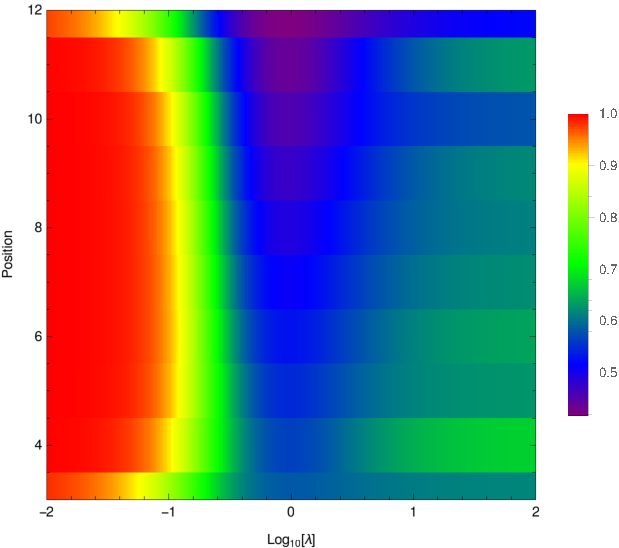
\includegraphics[width=1.0\textwidth]{TRM/images/analMidDensProfile}
  \end{center}
\end{figure}
 Looking at $\lambda=1$, we see that there is a roughly constant gradient for the density profile between the
 boundaries, which makes sense as this is the simple exclusion limit, so it's essentially just normal
 diffusion.
 As we go to smaller $\lambda$, we see that the system in general is quite full. Presumably this is because
 material has been sucked into the system due to the attraction implied by the small $\lambda$; this
 indicates that the boundaries used are a bit odd in this limit, as the system might not naturally form
 a homogeneous phase for such a $\lambda$ and could instead wish to form a mixture of lower and 
 higher density clumps, we will discuss this at greater length in Chap.~\ref{sec:numerics}.
 
 Our theory about why this occurs is as follows.
 At large 
 $\lambda$, we see that the density profile defaults to $\rho\sim\frac{2}{3}$ plus oscillations on the 
 boundaries which decay as we go towards the interior. This is suspiciously close to the critical density
 of the MFT (Chap.~\ref{sec:analChap}) which permits a maximal flow; therefore, we suggest that the system
 self-organises at high $\lambda$ to favour configurations that permit high current. The reason this density permits a high current is that in such a configuration,
 any particular particle should on average be in contact with an adjacent particle, with a free space to move into, so the dynamics of the system should be dominated by $\lambda$ rather than $1$. If the density were
 higher, some particles don't have spaces to move into, so that will slow things down; if the density were 
 lower, particles aren't receiving the speed benefit of being a neighbour. We believe that this 
 self-organisation occurs in the bulk, with thin boundary layers occurring near to boundaries
 with densities fixed away from $\frac{2}/{3}$ .
 We believe that this thin layer is revealed by the oscillatory layer observed near to the boundaries; right next to the boundary, in alternating sites, particles will tend to
 linger in sites where they are alone, rapidly leaving when they are prompted by the arrival of a new particle in 
 the  space next to them. This effect then smooths out as one goes deeper into the bulk.
 
 As for why a density which permitted fast flow would be favoured, consider what happens when a 
 region of low flow comes into contact with one of high flow: the high-flow region will invade the
 other region with particles or vacancies, raising the overall flow rate (which previously would
 have been limited by the slowest-flowing region) and thus flushing out or bringing in new 
 particles. In this way, the system as a whole will tend to favour the fast-flow densities, as
 they are more stable than the alternatives.
 
 \subsubsection{TRM-Computed Current} \label{sec:TRMLambdaScan}

 Whilst we computed the density profile, we also measured the steady state current. We also performed the
 same computation for different boundary conditions, and the results are displayed in Fig.\ref{fig:analCurr},
 along with the corresponding MFT prediction. Note that some of these calculations failed hence 
 the gaps in the spectra.
\afterpage{
 \begin{figure}[h!]
 \caption[The variation of the current (measured flowing from high density boundary to
 low) with $\lambda$ for a system of size
 $L=10$ and boundaries $(\rho_0 = 0.6, \rho_L = 0.4)$.]{\label{fig:analCurr} 
A logarithmic plot showing the variation of current with $\lambda$ in steady state for a system with boundary conditions $(\rho_0 , \rho_L )$ as indicated with system size $L=10$. 
The current measurement is oriented so that positive current corresponds to flow
from high density to low (the normal case). The relevant MFT prediction is shown via a dashed line in each
case.
 }
  \begin{center}
 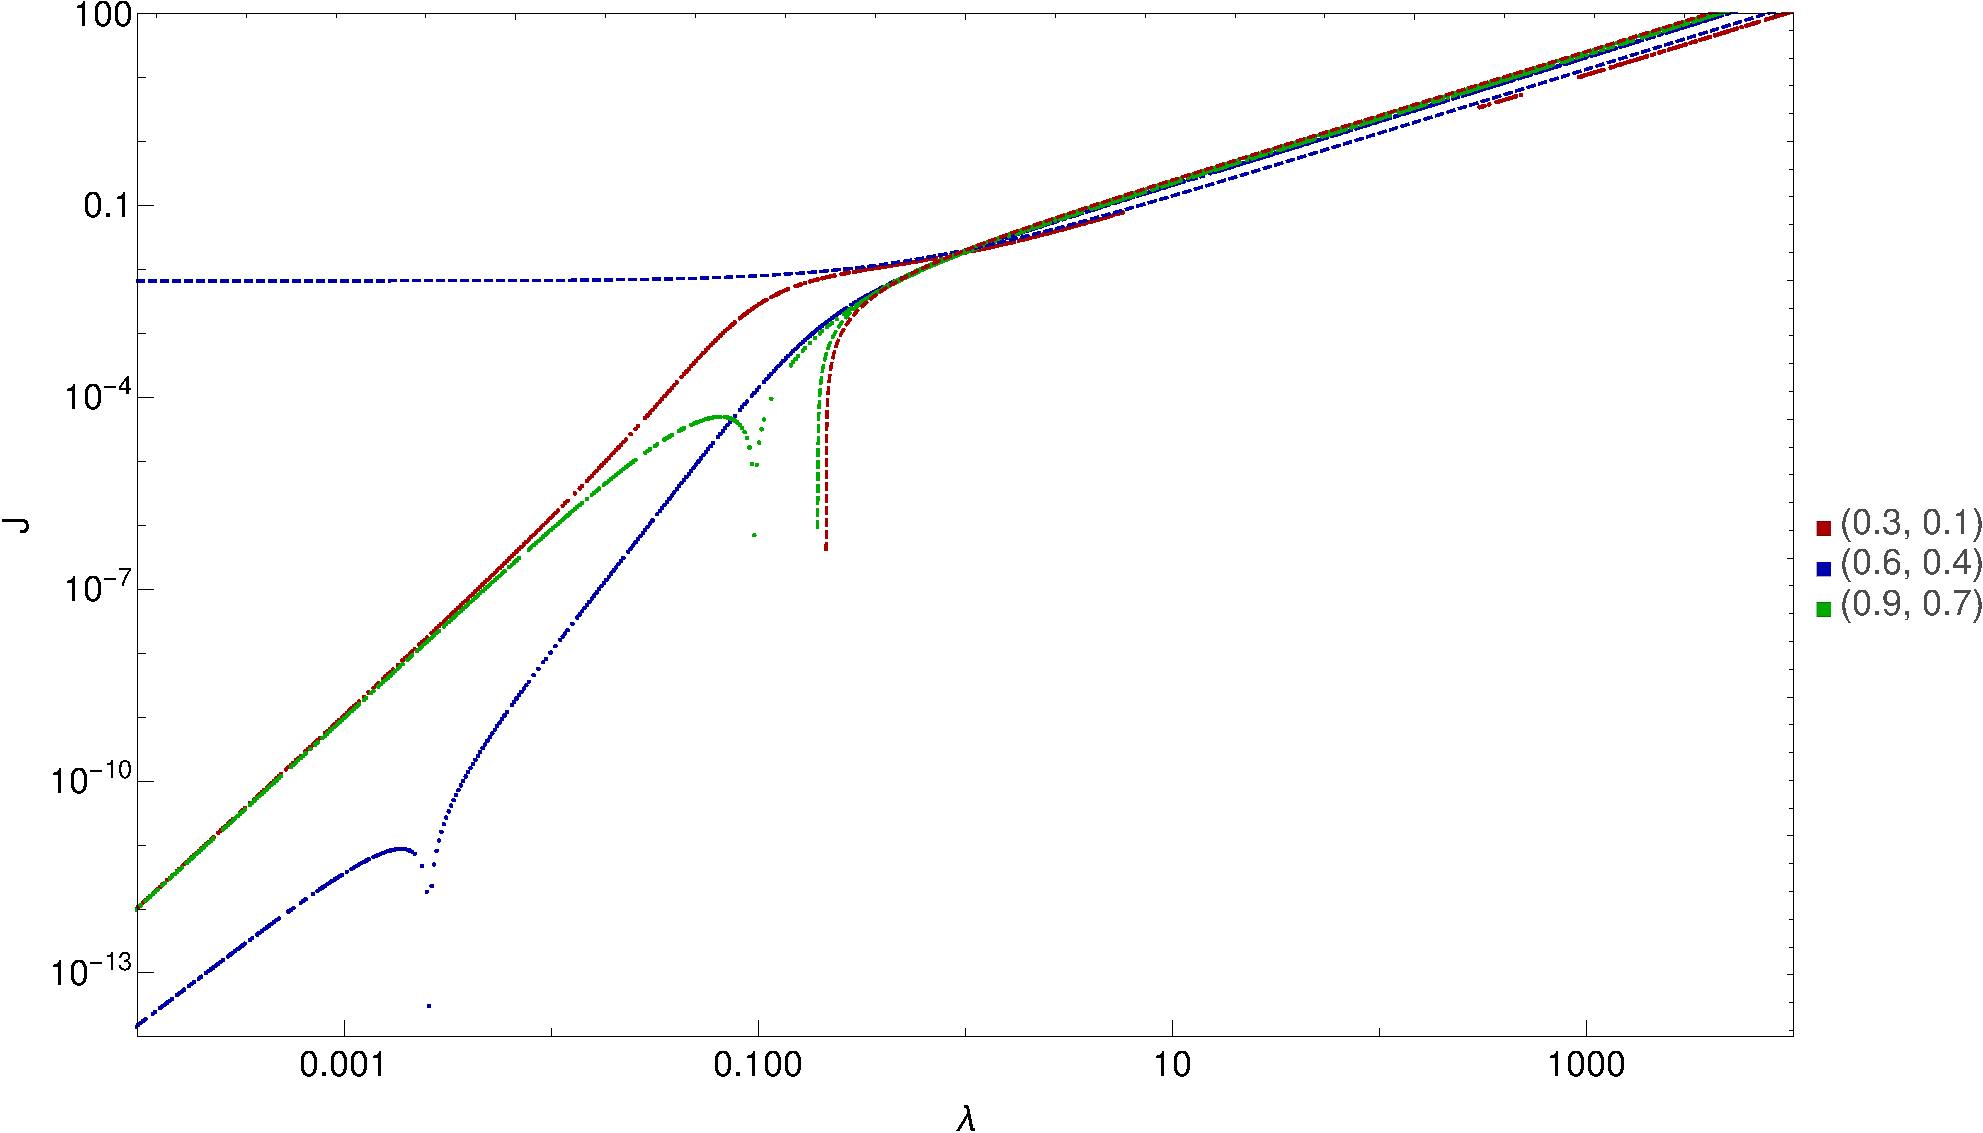
\includegraphics[width=0.9\textheight, angle=270]{TRM/images/TRMMFTCurrCombPlot}
  \end{center}
\end{figure}
\clearpage
}
There's a lot going on here, so let's break it down.
\begin{itemize}
 \item At large $\lambda$, we see that the scaling ($\mathcal{O}(\lambda)$) is the same for both the MFT
 and the TRM numerics. The actual values predicted by the MFT and the TRM calculations differ slightly,
 but not by a great deal until we have $\lambda < 1$. It is to be expected that there is a discrepancy,
 as the MFT is in the continuum-limit whereas the TRM system is only of size $L=10$. Furthermore, there
 should be a discrepancy anyway as the TRM system is not mean-field; it just doesn't seem to be so relevant
 in this regime.
 \item At $\lambda=1$, MFT and TRM calculations coincide, because the boundary conditions all differ
 by the same amount and $\lambda=1$ is the trivial case of simple exclusion.
 \item As we explore very small values of $\lambda$, we find that the MFT and the TRM have very little 
 resemblance. For boundary conditions $(0.3, 0.1)$ and $(0.9, 0.7)$ the MFT predicts that the flow should
 start running backwards or at the very least be pinned at zero,
 whilst for $(0.6, 0.4)$ it suggests that the current should tend to a constant
 as $\lambda \rightarrow 0$. 
 Instead of the flow crashing to zero, the TRM results show a more gradual reduction of the current.
 Measurement by comparison with a trendline shows that the current varies as $\mathcal{O}(\lambda^3)$ as 
 $\lambda$ becomes small.
 \item There is an intermediate regime in which the dependence of the current upon $\lambda$ transitions
 between $\mathcal{O}(\lambda^3)$ and $\mathcal{O}(\lambda)$. This is the situation for $\lambda \in (0.03, 0.5)$.
 \iffalse
 \item There is also some slightly odd behaviour on display in terms of the apparent ``poles'' in the 
 current for
the $(0.6, 0.4)$ and $(0.9, 0.7)$-boundaried systems. This could be due to a close-approach of eigenvalues,
causing the algorithm to pick the wrong one under certain circumstances. We have filtered the results by
imposing the inequality $\| q_0 \| \le \lambda K$ for $K=10^{-9}$ with $q_0$ being the ``zero'' eigenvalue,
but some results may have slipped through this net. We think this is the most likely explanation we have to
hand.
\fi
\end{itemize}
So, it seems that whilst we don't see a transition to zero flow as predicted by the MFT, we do see
a big change in the way the flow depends upon $\lambda$ as we pass between the large-$\lambda$ to 
small-$\lambda$ regimes.


\subsubsection{TRM-Computed Diffusion Coefficient}
It is also possible for us to compute an approximation to the effective diffusion coefficient.
Recall that the diffusion coefficient $D$ should satisfy
\begin{equation}
 \mathbf{J} = -D \mathbf{\nabla} \rho ;
\end{equation}
thus, we should be able to compute the diffusion coefficient using the TRM by computing the current $J$
with boundary conditions $(\rho_0, \rho_L) = (\rho+\frac{1}{2}\delta\rho, \rho-\frac{1}{2}\delta\rho)$,
and then evaluating the quantity
\begin{equation}
 D(\rho, \lambda) = \frac{L}{\delta \rho} J.
\end{equation}
We performed such a calculation, in which we picked $\delta \rho$ to be $0.001$ and $L=10$. We tabulated
$D$ for a range of $\lambda$ and $\rho$, and a contour plot of the data is displayed in 
Fig.~\ref{fig:TRMDiffCoeff}.
 \begin{figure}[h!]
 \caption[The variation of the diffusion coefficient of a system of size $L=10$ with respect to $\lambda$
 and $\rho$.]{\label{fig:TRMDiffCoeff} 
A coloured plot showing the variation of the diffusion coefficient with $\lambda$ and $\rho$
in steady state for a 
system of size $L=10$.
 }
  \begin{center}
 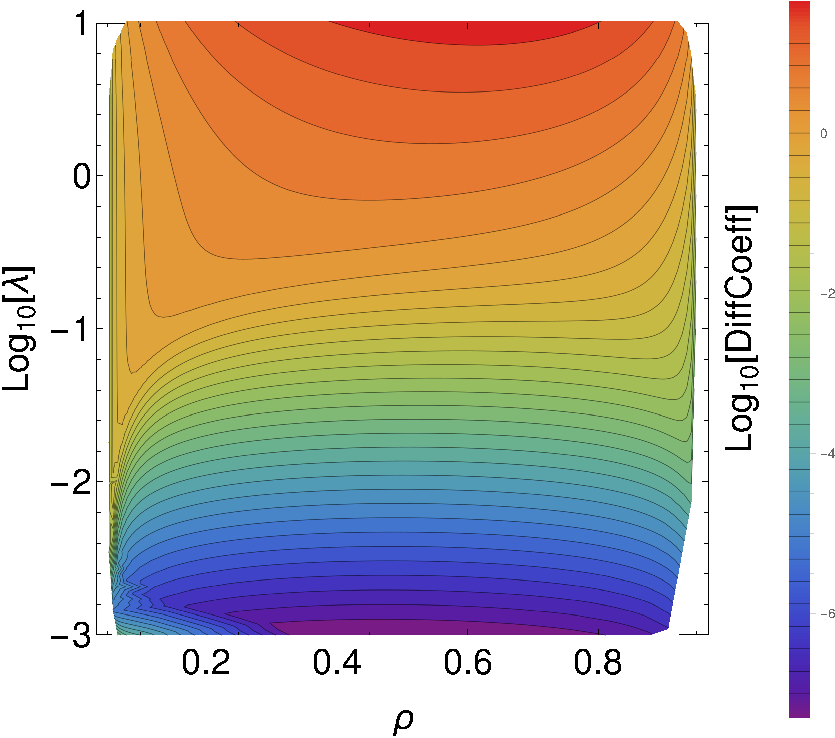
\includegraphics[width=1.0\textwidth]{TRM/images/TRMDiffCoeff}
  \end{center}
\end{figure}
In general, for given $\lambda<1$ we see that the variation with $\rho$ is usually pretty mild, with the more
extreme diffusion coefficients tending to occur for intermediate $\rho$. The exception to this occurs
primarily at small-$\lambda$, low density, where the diffusion 
coefficient is unusually high. This is presumably because the density
of particles is so low that the small value of $\lambda$ has little impact on the diffusion coefficient.
There is also some odd behaviour, in particular for extremely low $\lambda$ and low $\rho$. We probably
shouldn't trust those the results. As $\lambda \rightarrow 0$, the space of vectors with eigenvalue zero
switches from being $1$-dimensional to being very high-dimensional, because any state containing adjacent
particles becomes a steady state (and in fact an absorbing state). Thus, we should expect that at some
as we go to smaller and smaller $\lambda$ our calculations should start behaving badly because the lower
nonzero  eigenvalues become numerically indistinguishable from the actual zeros, and that is probably what
is happening here.
For $\lambda>1$, we see that maximal flow for a given $\lambda$ occurs for intermediate values of
$\rho$, consistent with the normal SEP result for $\lambda=1$. We can see that as $\lambda$
becomes large, the maximal flow density drifts towards $\rho=\frac{2}{3}$; this agrees with our
notion, backed by the MFT, that maximal flow at large-$\lambda$ should occur for
$\rho=\frac{2}{3}$.

The trend in terms of $\lambda$ is that the gradient of the diffusion coefficient as it varies with 
$\lambda$ and $\rho$ is generally low for large $\lambda$ and high for small $\lambda$. In light
of our results in Fig.~\ref{fig:analCurr}, this makes sense as the power law seems to change as we switch
between low and high $\lambda$. This suggests that an order parameter of the form
\begin{equation}
 \chi(\rho, \lambda) = \left(\partDeriv{\ln{D}}{\ln{\lambda}}\right)_\rho
\end{equation}
should reveal the power-law structure. We can compute this from our existing data in Fig.
\ref{fig:TRMDiffCoeff}, and it is displayed in Fig.~\ref{fig:TRMOrderParam}.
 \begin{figure}[h!]
 \caption[The variation of the order parameter $\chi$ for a system of size $L=10$ with respect to $\lambda$
 and $\rho$.]{\label{fig:TRMOrderParam} 
A coloured plot showing the variation of the order parameter $\chi$ with $\lambda$ and $\rho$
in steady state for a 
system of size $L=10$.
 }
  \begin{center}
 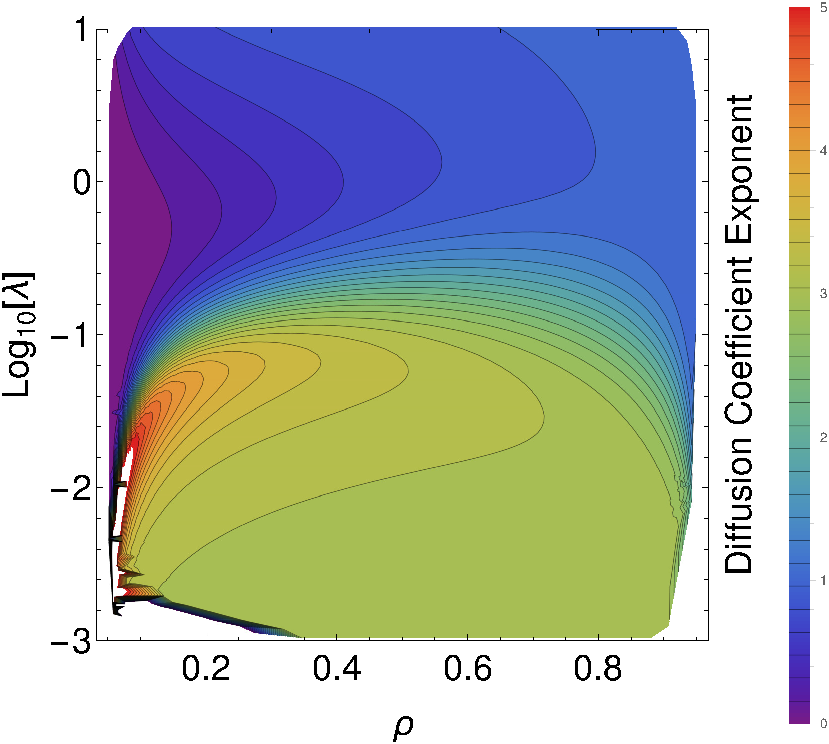
\includegraphics[width=1.0\textwidth]{TRM/images/TRMOrderParam}
  \end{center}
\end{figure}
As you can see, this order parameter does seem to nicely partition $(\rho, \lambda)$ space into two
components, divided by a region of extremely rapid change. The order parameter $\chi$ could be regarded as
some kind of susceptibility. An issue here is that it is hard to see how $\chi$'s apparent transition
will vary with system size, as $L=10$ is a very small system, and transitions only become sharp in the
limit of large systems. We could of course use it in a Monte-Carlo calculation in a larger system, but
then we have the problem that it's difficult to take meaningful derivatives of noisy data. We will leave
it, then, as a curiosity.

\section{Time-Dependent Properties of Small SPM Systems}
Although we have mostly concentrated on calculating steady state properties of the SPM, it is also possible to calculate some dynamical properties. 
\subsection{The Relaxation Time for the SPM} \label{sec:relaxTime}
As we have seen, the eigenvalue with least negative real
part effectively controls the rate at which a generically-prepared system equilibrates, by acting as a lower bound on the rate of relaxation towards equilibrium. Therefore, the reciprocal of this 
relaxation rate should yield a characteristic time for convergence to equilibrium, the relaxation
time. We have computed this relaxation time for
our three standard boundary conditions in Fig.~\ref{fig:TRMRelaxTime}.
 \begin{figure}[h!]
 \caption[The dependence of the relaxation time on $\lambda$ for three sets of boundary conditions.]{\label{fig:TRMRelaxTime} 
A plot showing the dependence of the relaxation time upon $\lambda$ for a system of size $L=10$ with
boundary densities $(0.3, 0.1)$, $(0.6, 0.4)$ and $(0.9, 0.7)$. In terms of units, here we are presuming that the default diffusion rate $\tau_0 = 1 \mathrm{s}^{-1}$.
 }
  \begin{center}
 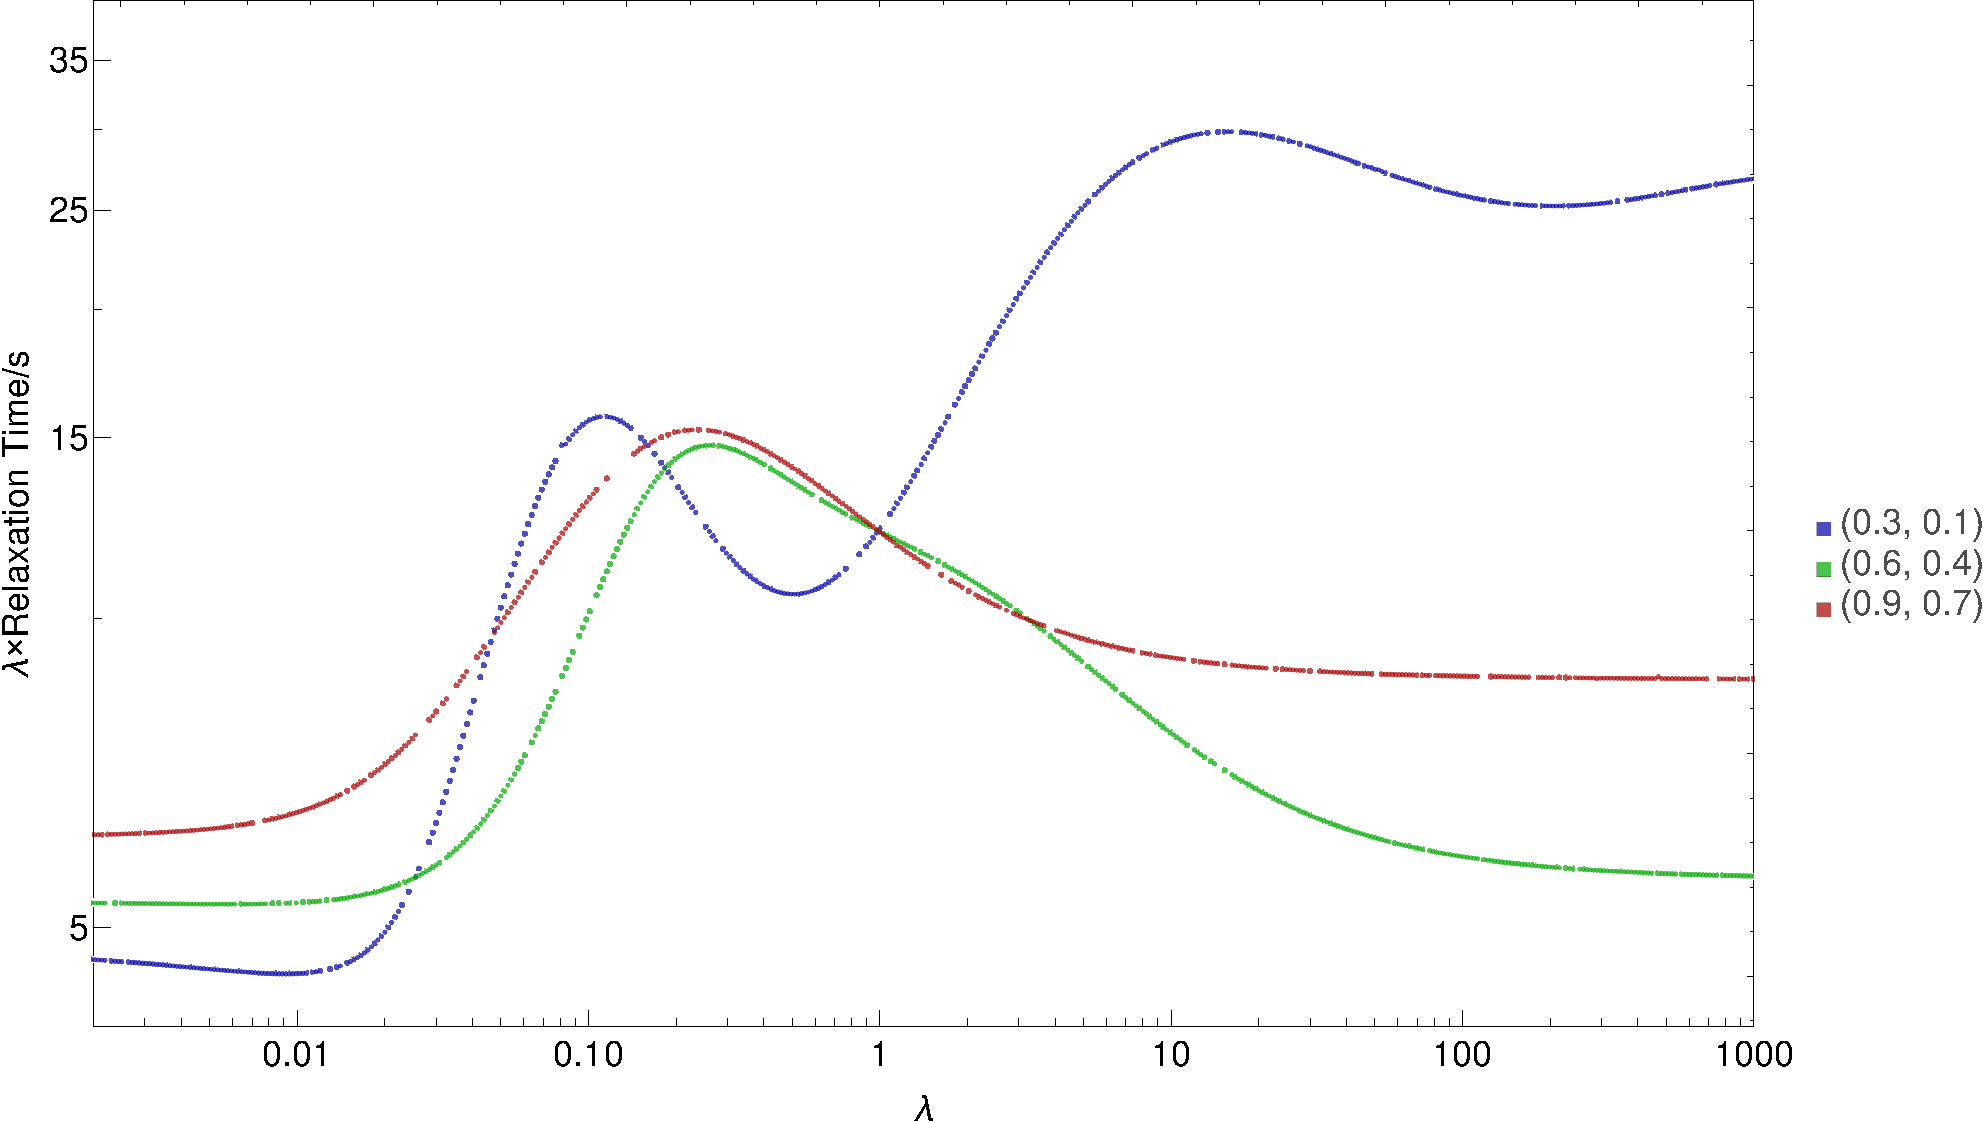
\includegraphics[width=1.0\textwidth]{TRM/images/TRMRelaxTime}
  \end{center}
\end{figure}
Notice first that we have plotted the relaxation time multiplied by $\lambda$, as the relaxation time
generally scales as $\mathcal{O}(\lambda^{-1})$. One can see why we made this choice by looking at the
extremes, where the lines are generally quite flat.

Observe that the relaxation times for large $\lambda$ are generally a little higher than for low 
$\lambda$ once the $\mathcal{O}(\lambda^{-1})$ dependence is taken into account. In particular, the
system with low densities at the boundary is much slower to relax to equilibrium than the system with high boundary densities, which in turn is slow compared to the system with medium densities. This is
presumably because the system is attempting to reach the maximal flow density we observed, $\rho = \frac{2}{3}$, and it finds it more awkward to do that the further away the furthest boundary is from
$\frac{2}{3}$.

For very low $\lambda$, the difference between boundary configurations isn't so great, and we believe
that the differences between the boundaries occur for the same reason as for the high-$\lambda$
situation, only now the system is trying to fill instead of hold at $\rho=\frac{2}{3}$. For intermediate
$\lambda$, things are less clear. At $\lambda=1$, all systems equilibrate at the same rate; other than
that, behaviour varies pretty wildly. Equilibration time is generally on the high side for
$\lambda \in (0.03, 1)$, which is where the current looks like its undergoing some kind of
transition, so this increase in relative equilibration time could be interpreted as an accumulation of
fluctuations in that regime.
\subsection{Time-Evolution of States}
Recall from Sec.~\ref{sec:TRMGeneralResults} that the Master Equation (Eq.~\ref{eq:masterEq}) has
a formal solution given by Eq.~\ref{eqn:formalSoln}, in which we premultiply the initial state
by a matrix exponential of the TRM. Throughout this chapter we have been making use of the fact that
the TRM is sparse in order to perform our computations. Thus, it would seem that we couldn't
investigate the time evolution of systems, as $e^A$ is in general not sparse even if $A$ is sparse,
and thus we would instantly run out of memory if we tried to compute anything.

However, the premultiplication of a vector by a sparse matrix can be performed \textit{in place},
and this is implemented by Python's routine \texttt{scipy.sparse.linalg.expm\_multiply}. Therefore
we have been able to calculate the time-evolution of arbitrary initial distributions. By way of an
example we prepared three systems with initial uniform distributions, in which all possible 
configurations are equally likely, and then monitored how their spatial occupations varied as they
relaxed towards equilibrium (which should always occur, as discussed in 
Sec.~\ref{sec:TRMGeneralResults}). The results are displayed in Fig.~\ref{fig:TRMTimeDep}.
\begin{figure}
\caption[The time-evolution of uniform distributions to equilibrium.]{Plots of the time-evolution
of the density profiles of systems prepared with uniform distributions. These systems are of
size $L=10$, with boundary densities $(0.9, 0.1)$, $b_0=100.0$ and $\lambda= \{ 0.1, 1.0, 2.0 \}$,
going from top to bottom, respectively. The total time intervals have been adjusted to suit the 
equilibration time.} \label{fig:TRMTimeDep}
\begin{center}
 \begin{tabular}{c}
    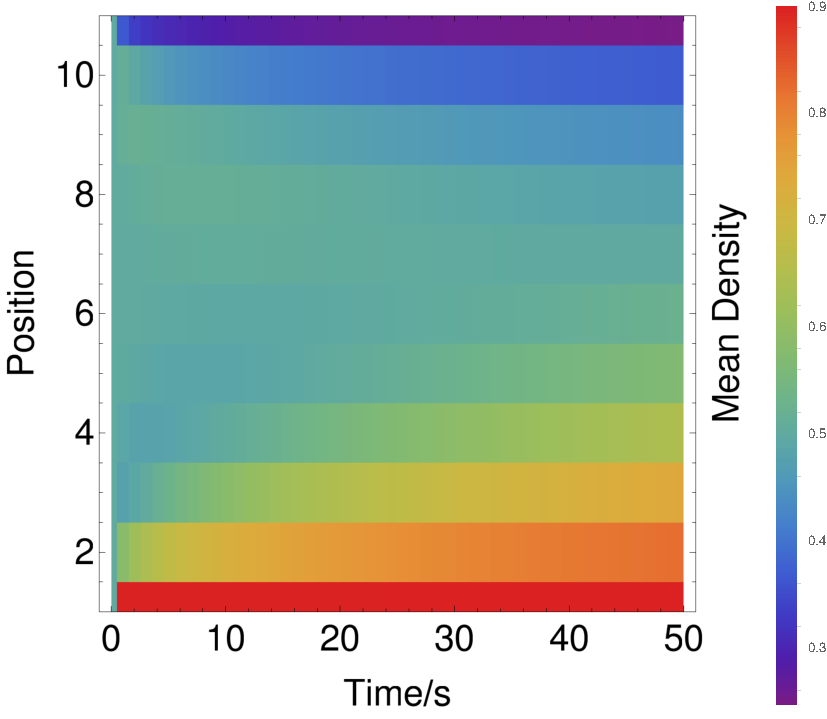
\includegraphics[width=0.6\linewidth]{TRM/images/timeSeriesl0_1}  \\ 
    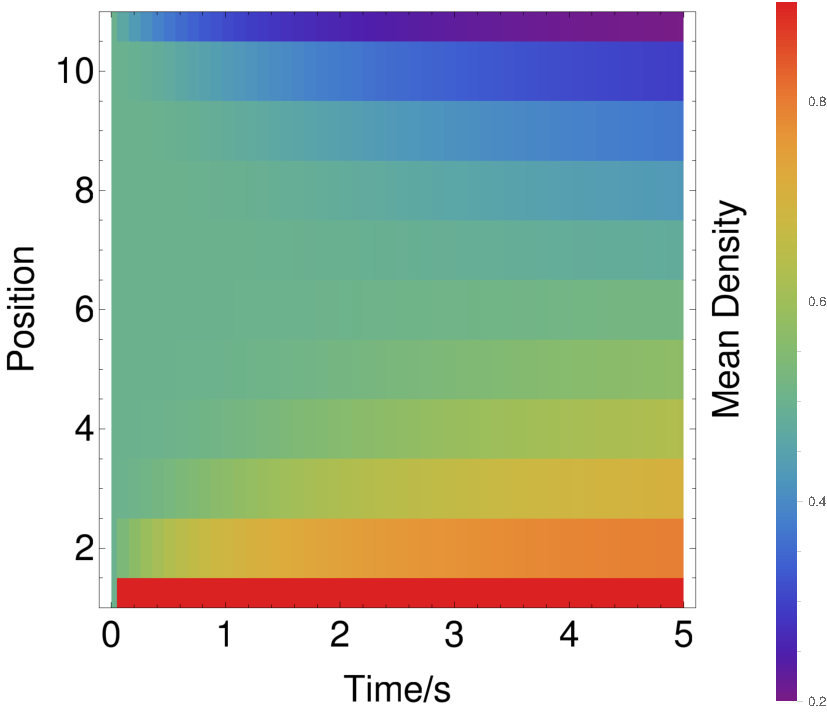
\includegraphics[width=0.6\linewidth]{TRM/images/timeSeriesl1_0}  \\
    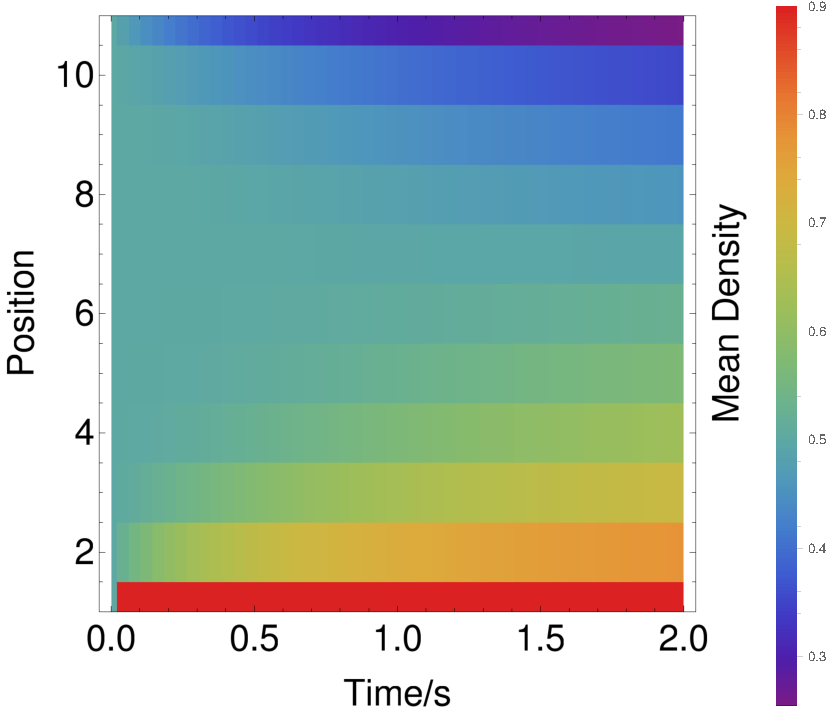
\includegraphics[width=0.6\linewidth]{TRM/images/timeSeriesl2_0}  \\
    \end{tabular}
\end{center}
    \vspace{-2em}
\end{figure}
In the plots we have included the innermost site in the boundary layer; notice that it switches to the 
``correct''
mean occupation almost instantly, which is exactly what is supposed to happen as it represents a highly
responsive reservoir. The system then gradually makes its ways toward equilibrium, starting at the 
boundaries and working inward, and the characteristic timescale over which this occurs seems to be in
line with our results from \ref{sec:relaxTime}.

Of course, this is more of a demonstration of what this method could achieve than actually useful
results. We are quite sure that with a little effort one could use it to calculate time-dependent
spatial correlation functions,
for example, but we simply worked out how to perform TRM calculations too late in the project to be
able to use it to full effect.


\section{Conclusions}

Numerically approximating the eigenpairs of the transition rate matrix is a convenient
alternative to the use of
Monte Carlo methods for the computation of the properties of a Markovian statistical mechanics system.
When using the TRM, we sacrifice system size for accuracy, as the memory requirement for TRM
calculations scales exponentially with system size, whilst similar Monte Carlo calculations scale 
linearly. However, the TRM method avoids the
sampling issues which often emerge when attempting Monte Carlo simulations, and can yield the relevant
statistics with relative ease once the matrix computations are completed. Furthermore, we can also
investigate time-dependent properties at our convenience, which can be awkward in Monte-Carlo 
calculations as there we don't usually work with normal time.

The main reason we performed these calculations, however, is to investigate the current flowing due
to the boundary conditions. We found that the MFT prediction that the currents drops to zero or becomes 
negative below a critical $\lambda$ (depending upon boundary conditions) does not seem to be correct;
however, we have found that the scaling of the current does seem to undergo some kind of transition,
from  $J \propto \lambda$ for high $\lambda$ to $J \propto \lambda^3$. This is something which we can
investigate further using Monte-Carlo methods on larger-scale systems, and we will do this in the next
chapter.
